\documentclass[12pt,letterpaper,oneside,reqno]{amsart}
\usepackage{amsfonts}
\usepackage{amsmath}
\usepackage{amssymb}
\usepackage{amsthm}
\usepackage{float}
\usepackage{mathrsfs}
\usepackage{colonequals}
\usepackage[font=small,labelfont=bf]{caption}
\usepackage[left=1in,right=1in,bottom=1in,top=1in]{geometry}
\usepackage[pdfpagelabels,hyperindex,colorlinks=true,linkcolor=blue,urlcolor=magenta,citecolor=green]{hyperref}
\usepackage{setspace}
\usepackage{graphicx}
\usepackage{spverbatim}
\pdfminorversion=7
\linespread{1.7}
\emergencystretch=1em
\apptocmd{\sloppy}{\hbadness 10000\relax}{}{}
\raggedbottom

% free foot note
\let\svthefootnote\thefootnote
\newcommand\freefootnote[1]{%
    \let\thefootnote\relax%
    \footnotetext{#1}%
    \let\thefootnote\svthefootnote%
}


\title[.NET Core Web API Azure Ubuntu Virtual Machine deployment manual]
{.NET Core Web API Azure Ubuntu Virtual Machine deployment manual}
\author[Petro Kolosov]{Petro Kolosov}
\email{kolosovp94@gmail.com}
\keywords{
    Azure, Ubuntu Server, ASP.NET Core, Web API, Nginx, Let's Encrypt, SSL certificates, Cloudflare,
    DNS management, reverse proxy.
}
\urladdr{https://kolosovpetro.github.io/}
\date{\today}
\hypersetup{
    pdftitle={.NET Core Azure Ubuntu VM deploy guide},
    pdfsubject={
        Azure, Ubuntu Server, ASP.NET Core, Web API, Nginx, reverse proxy, Let's Encrypt, CertBot, SSL certificates,
        Cloudflare, DNS management, VM provisioning, API deployment, HTTPS setup, scalable deployment,
        secure web application, cloud deployment, Azure VM, web server configuration, domain integration
    },
    pdfauthor={Petro Kolosov},
    pdfkeywords={
        Azure, Ubuntu Server, ASP.NET Core, Web API, Nginx, reverse proxy, Let's Encrypt, CertBot, SSL certificates,
        Cloudflare, DNS management, VM provisioning, API deployment, HTTPS setup, scalable deployment,
        secure web application, cloud deployment, Azure VM, web server configuration, domain integration
    }
}
\begin{document}
    \begin{abstract}
        This document provides a comprehensive guide on deploying an ASP.NET Core Web API on an Azure Ubuntu Server virtual
machine (VM).
The deployment process leverages Nginx as a reverse proxy,
while secure HTTPS connection is being configured by using Let's Encrypt CertBot free SSL certificates.
Additionally, domain name (DNS) management is handled by utilizing Cloudflare.
This guide covers the end-to-end setup, including VM provisioning, API deployment, SSL configuration, and domain integration,
ensuring a secure, scalable, and high-performance web application environment on Azure.

    \end{abstract}

    \maketitle

    \tableofcontents

    \freefootnote{Sources: \url{https://github.com/kolosovpetro/AzureUbuntuVMDeploy}}


    \section{Virtual machine creation}\label{sec:virtual-machine-creation}
    Firstly, it is necessary to create a virtual machine (unexpectedly) where deployment to be hosted on.
In this guide is considered free virtual machine of type \texttt{Standard B1ms (1 vcpu, 2 GiB memory)}
with Ubuntu 20.04 operating system.
Definitely it won't be considered step by step creation in this document, however required VM parameter are as follows:
\begin{itemize}
    \item Size: \texttt{Standard B1ms (1 vcpu, 2 GiB memory)}
    \item OS: \texttt{Ubuntu Server 20.04 LTS - Gen2}
    \item Availability options: \texttt{No infrastructure required}
    \item Authentication type: \texttt{SSH public key}
    \item SSH public key source: \texttt{Use existing public key (create it before you created VM)}
    \item Public inbound ports: \texttt{HTTP(80), HTTPS(443), SSH(22)}
    \item OS disk type: \texttt{Standard SSD}
    \item Encryption type: \texttt{Default}
    \item Public IP: \texttt{Basic SKU, Static (be sure to create static IP)}
    \item Select inbound ports: \texttt{HTTP(80), HTTPS(443), SSH(22)}
    \item Boot diagnostics: \texttt{Disabled}
\end{itemize}
Chosen parameters of the virtual machine are collected in order to minimize vm's cost.
If you are not sure, refer to the screenshots via the reference~\cite{Create_Vm_Screens}.


    \section{Connect to VM via SSH}\label{sec:connect-to-vm-via-ssh}
    In order to configure virtual machine manually (as this guide tends to describe),
we have to connect to it via SSH using the specified RSA private and public key-pair.
It is assumed that programmer uses \texttt{WSL2} under \texttt{Windows 10} in order to work with VM via the SSH\@.
By default, SSH keys are stored under the path \texttt{c/Users/username/.ssh}.
Assume that RSA key-pair is stored there and have the names \texttt{id\_rsa} and \texttt{id\_rsa.pub} for private
and public keys respectively.
In order to interact the VM via SSH it is necessary to copy RSA keypair to the WSL \texttt{username/.ssh} folder,
we use the commands under WSL
\begin{itemize}
    \item \texttt{cp /mnt/c/Users/pkolosov/.ssh/id\_rsa ~/.ssh/}
    \item \texttt{cp /mnt/c/Users/pkolosov/.ssh/id\_rsa.pub ~/.ssh/}
\end{itemize}
Then connection is available now using the command
\begin{itemize}
    \item \texttt{ssh -i ~/.ssh/id\_rsa razumovsky\_r@MachineStaticIP}
\end{itemize}
\begin{figure}[H]
    \centering
    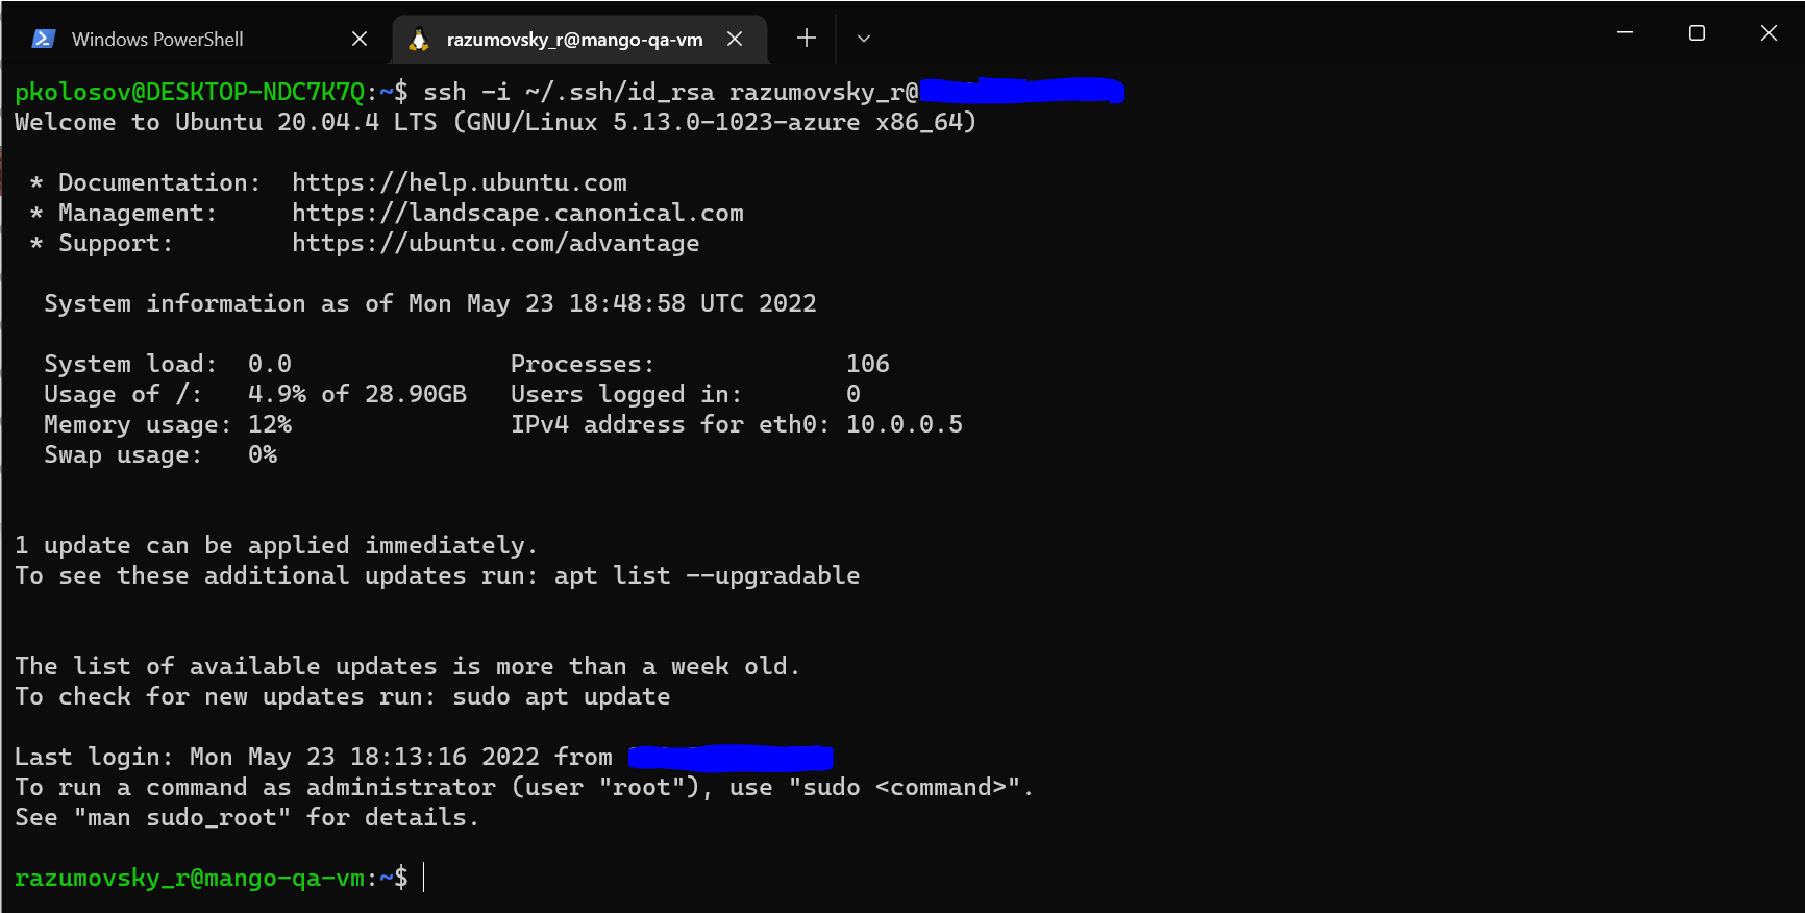
\includegraphics[width=1\textwidth]{img/01_ssh_connected}
    ~\caption{SSH connected successfully.}\label{fig:figure}
\end{figure}



    \section{Install .NET SDK and Runtime to the Ubuntu 20.04}\label{sec:install-.net-sdk-to-ubuntu-20.04}
    Next, we should install the .NET SDK (unexpectedly again) in order to run our application.
Proceeding, we refer to the Microsoft documentation article named
\href{https://docs.microsoft.com/en-us/dotnet/core/install/linux-ubuntu}
{\texttt{Install the .NET SDK or the .NET Runtime on Ubuntu}}~\cite{MSDN_Ubuntu}, precisely the version is 20.04.
As per documentation, consider the following commands to install .NET 6.0 SDK to your Ubuntu VM
\begin{figure}[H]
    \centering
    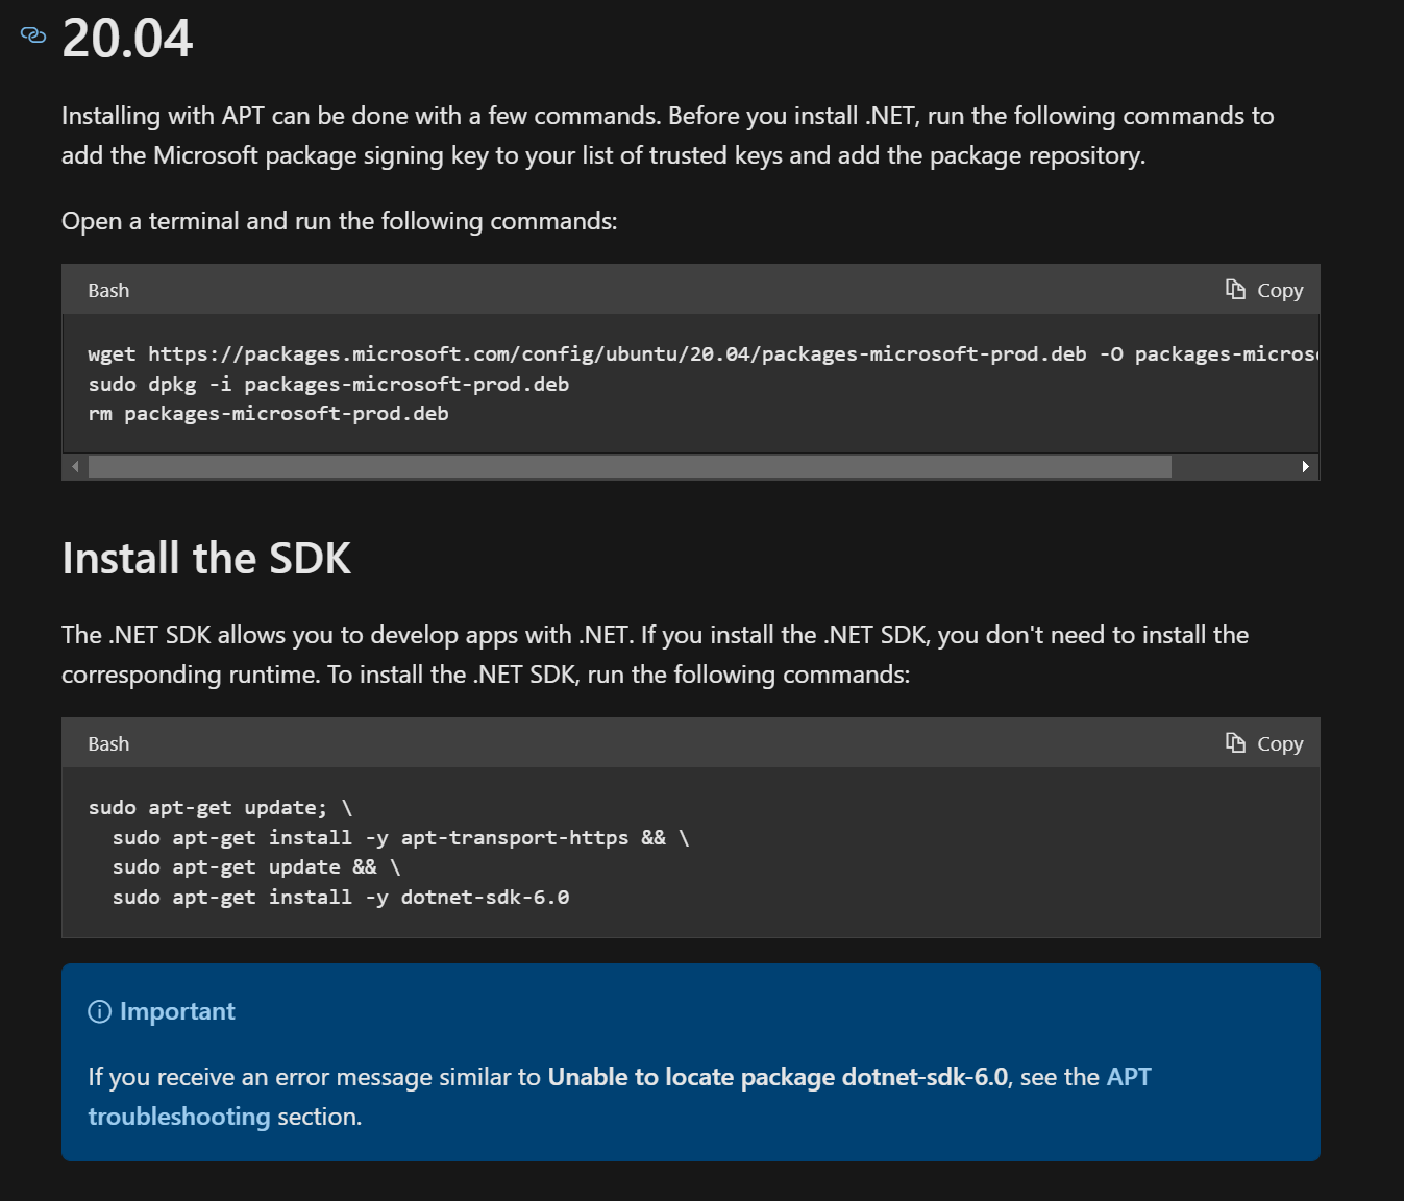
\includegraphics[width=1\textwidth]{img/03_1_sdk_documentation}
    ~\caption{Ubuntu 20.04 install .NET 6.0 SDK MSDN.}\label{fig:figure2}
\end{figure}
Prepare your virtual machine applying the commands
\begin{itemize}
    \item \texttt{wget https://packages.microsoft.com/config/ubuntu/20.04/packages-microsoft-prod.deb -O packages-microsoft-prod.deb}
    \item \texttt{sudo dpkg -i packages-microsoft-prod.deb}
    \item \texttt{rm packages-microsoft-prod.deb}
\end{itemize}
The terminal output is as follows
\begin{figure}[H]
    \centering
    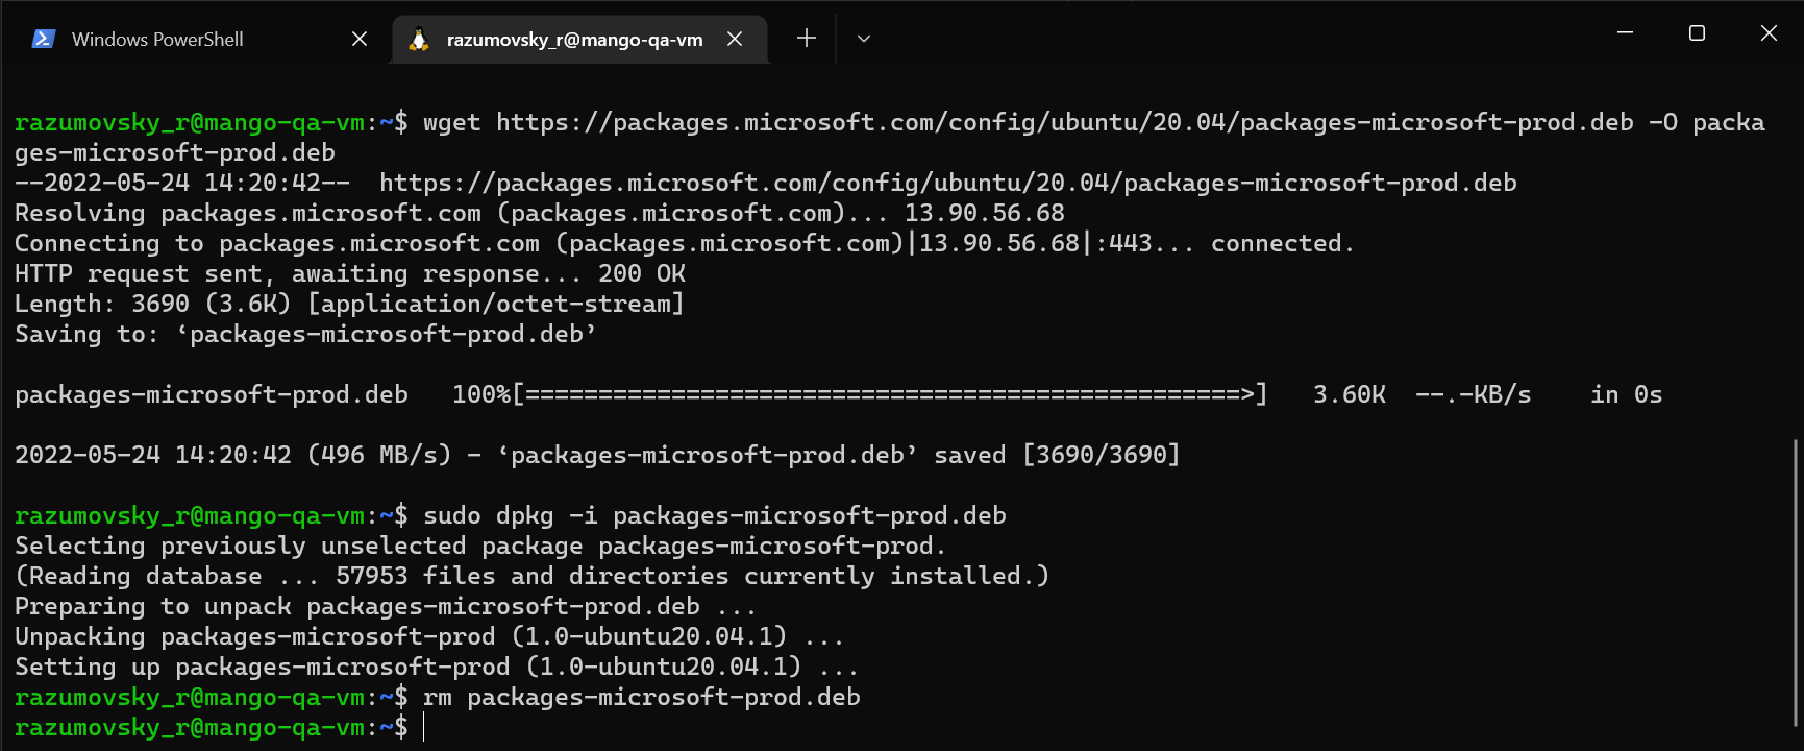
\includegraphics[width=1\textwidth]{img/03_3_vm_prepare}
    ~\caption{Virtual machine preparation..}\label{fig:figure3}
\end{figure}
Apply the following commands in order to install the SDK
\begin{itemize}
    \item \texttt{sudo apt-get update}
    \item \texttt{sudo apt-get install -y apt-transport-https}
    \item \texttt{sudo apt-get update}
    \item \texttt{sudo apt-get install -y dotnet-sdk-6.0}
\end{itemize}
The terminal output after .NET 6.0 SDK installation is as follows
\begin{figure}[H]
    \centering
    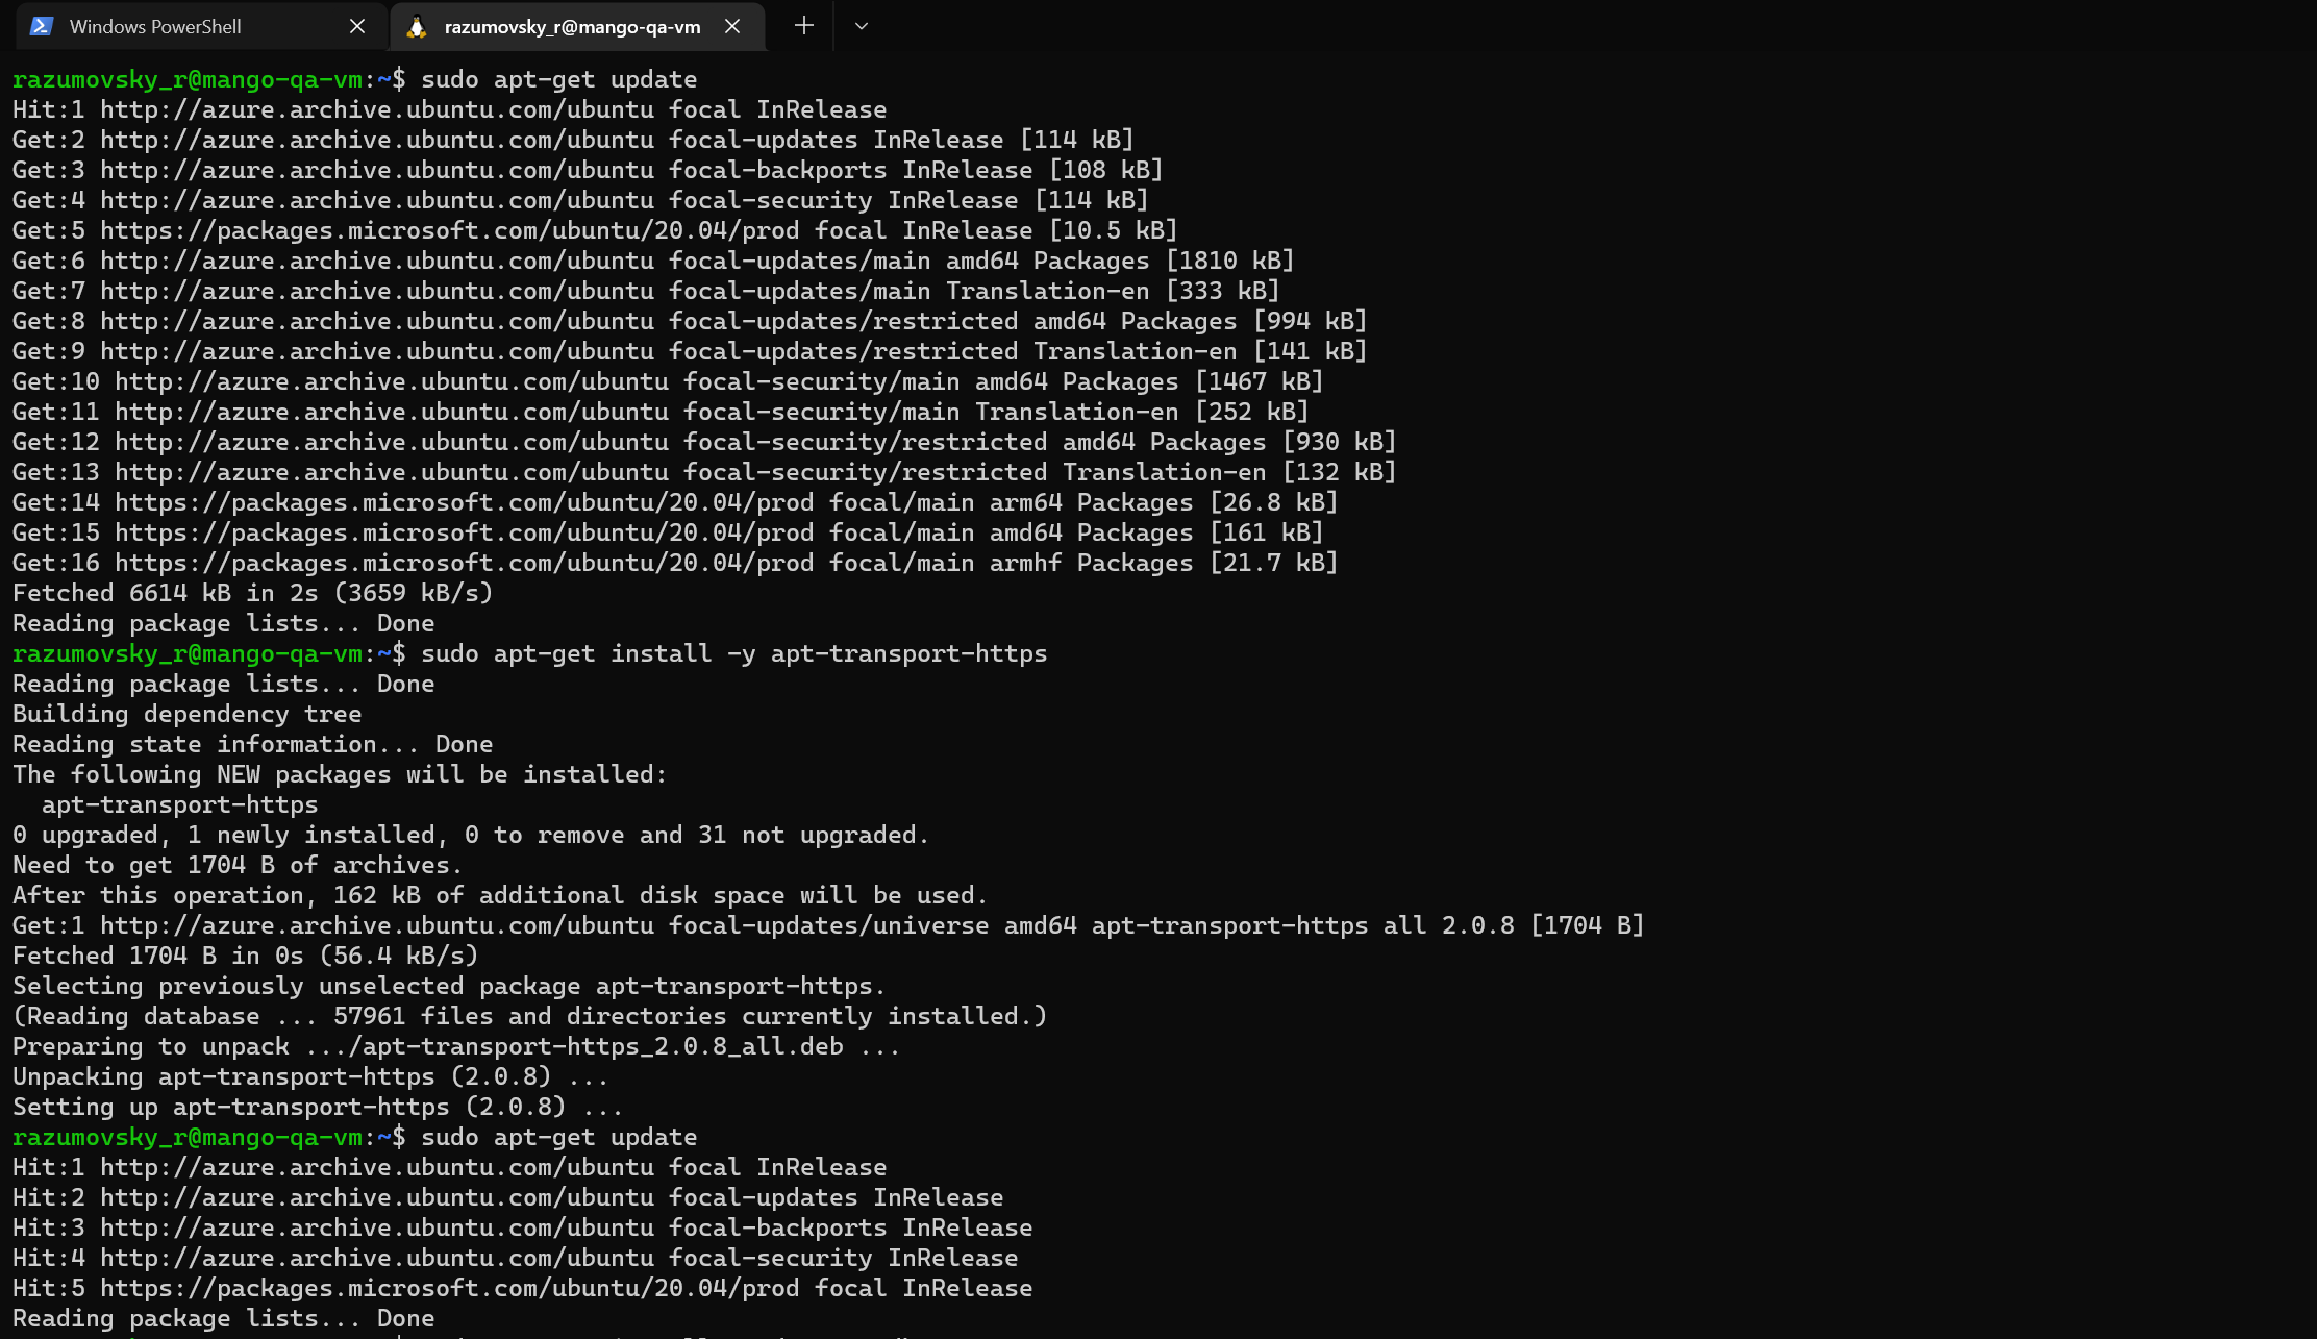
\includegraphics[width=1\textwidth]{img/03_4_sdk_install_1}
    ~\caption{Ubuntu 20.04 install .NET 6.0 SDK terminal output.}\label{fig:figure4}
\end{figure}
\begin{figure}[H]
    \centering
    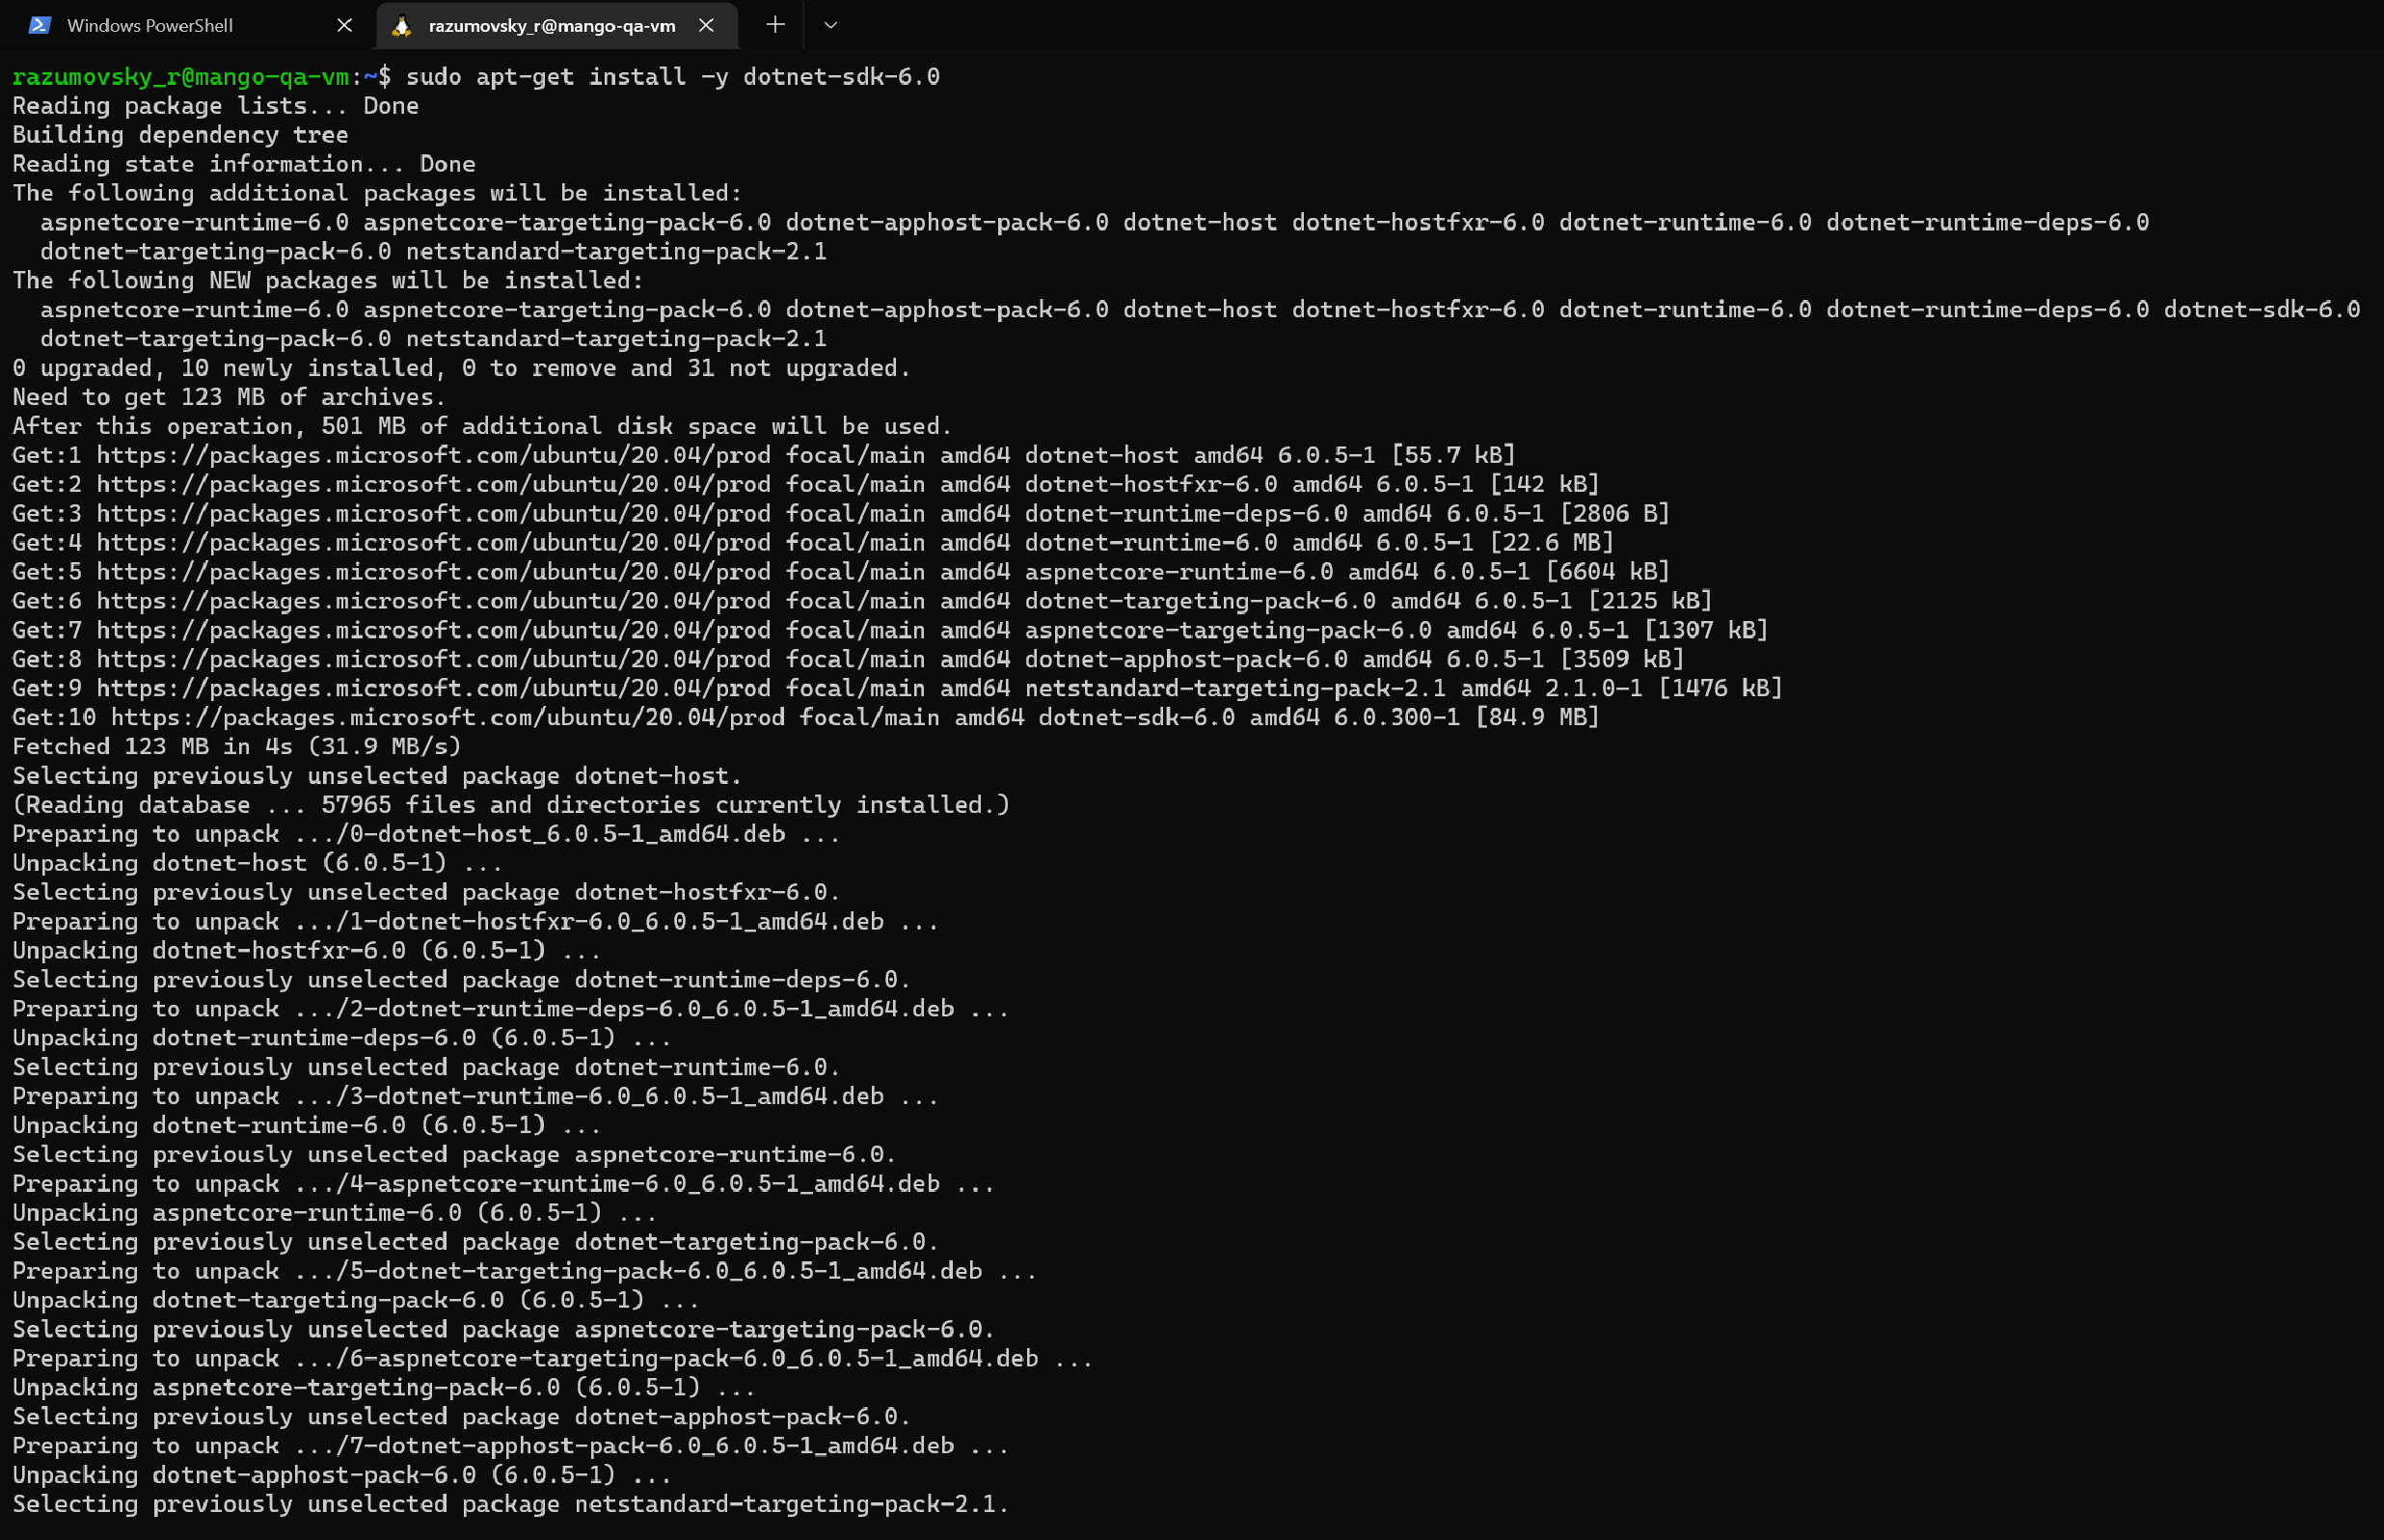
\includegraphics[width=1\textwidth]{img/03_4_sdk_install_2}
    ~\caption{Ubuntu 20.04 install .NET 6.0 SDK terminal output.}\label{fig:figure5}
\end{figure}
\begin{figure}[H]
    \centering
    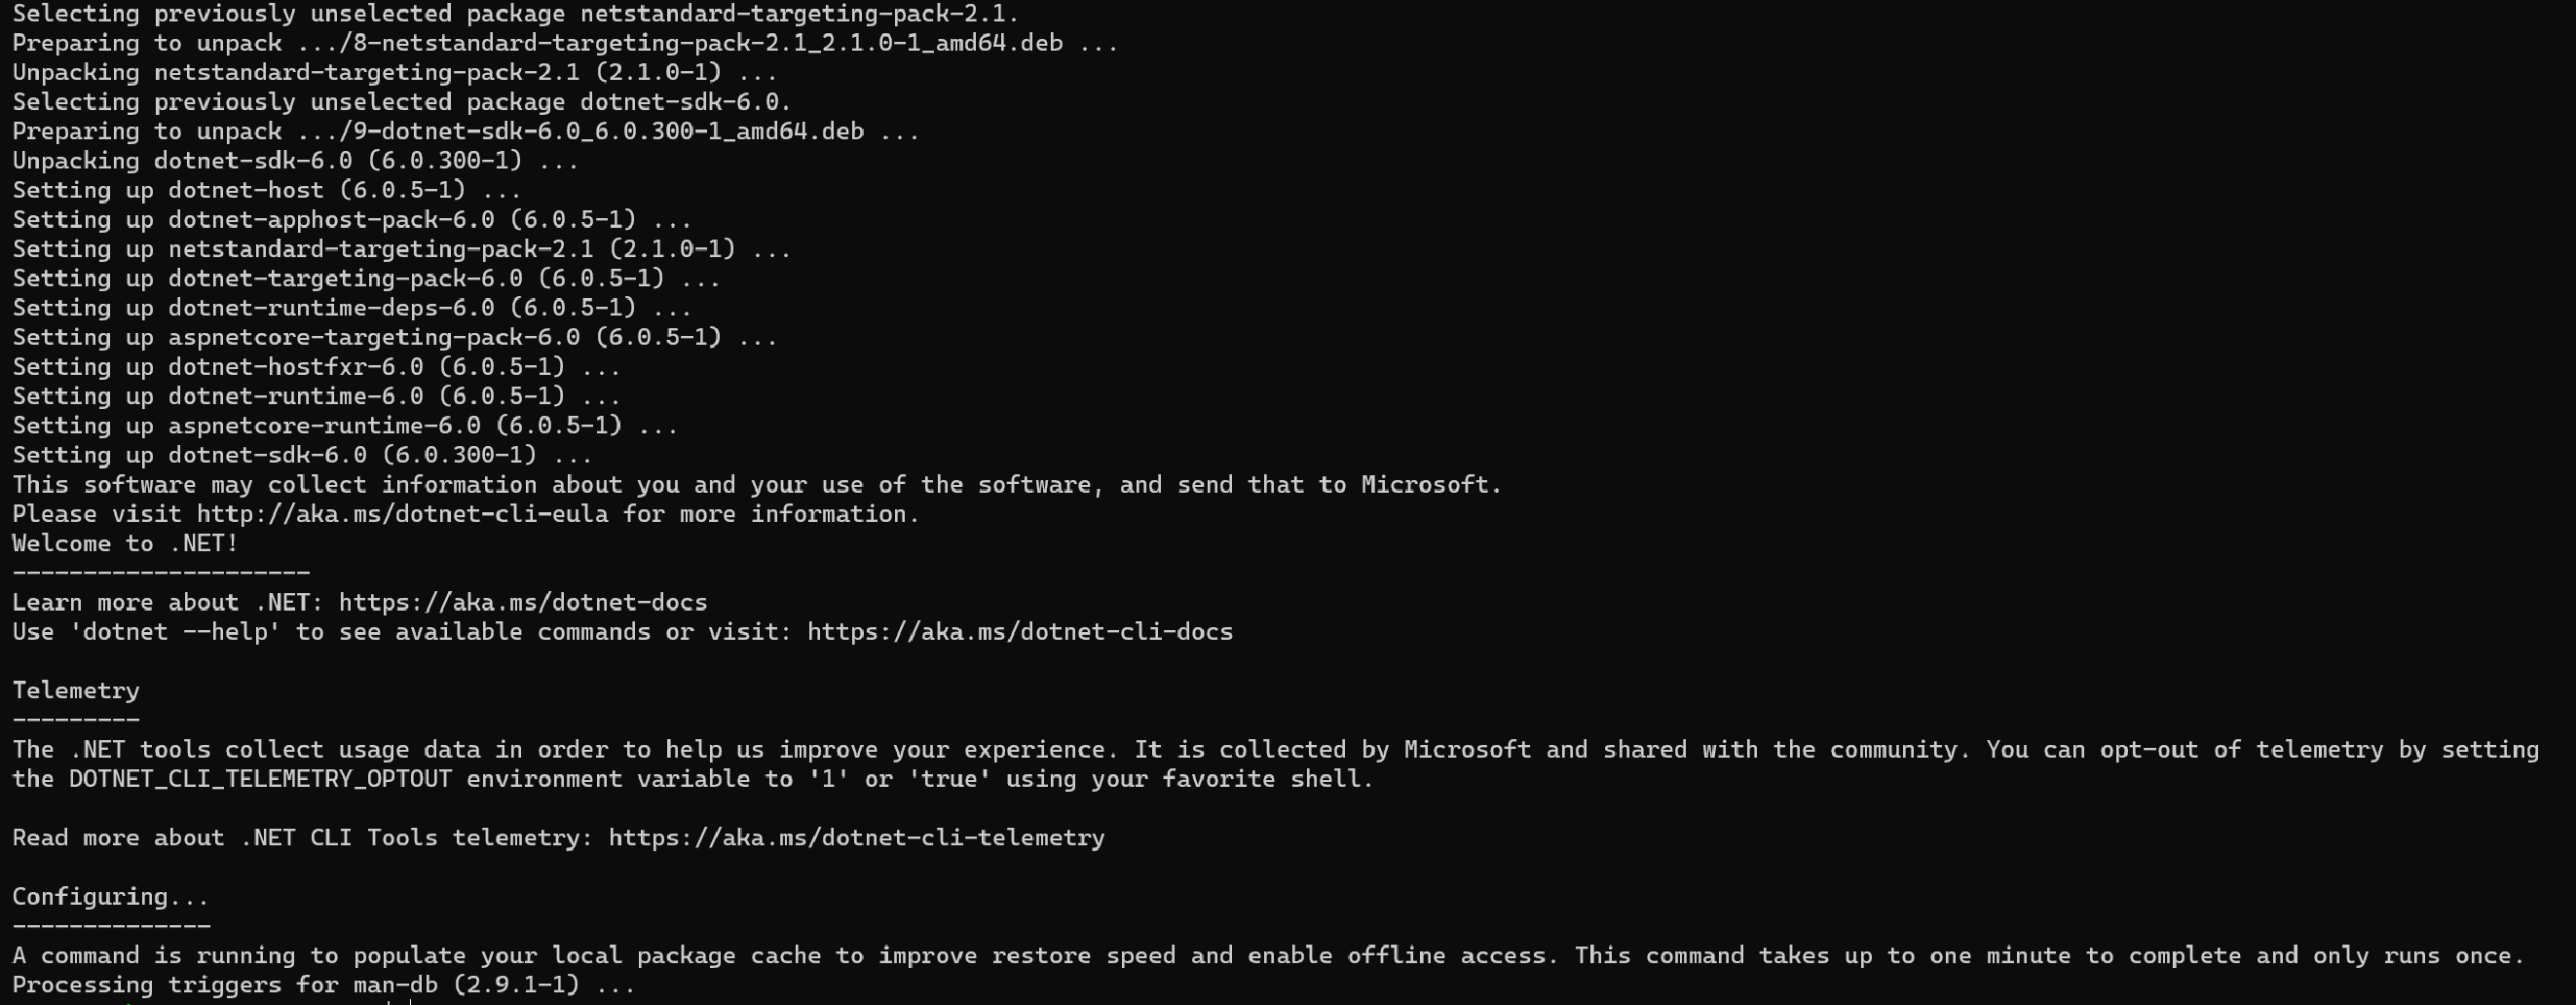
\includegraphics[width=1\textwidth]{img/03_4_sdk_install_3}
    ~\caption{Ubuntu 20.04 install .NET 6.0 SDK terminal output.}\label{fig:figure6}
\end{figure}

In order to install the .NET Runtime we refer again to the Microsoft documentation, that is
\begin{figure}[H]
    \centering
    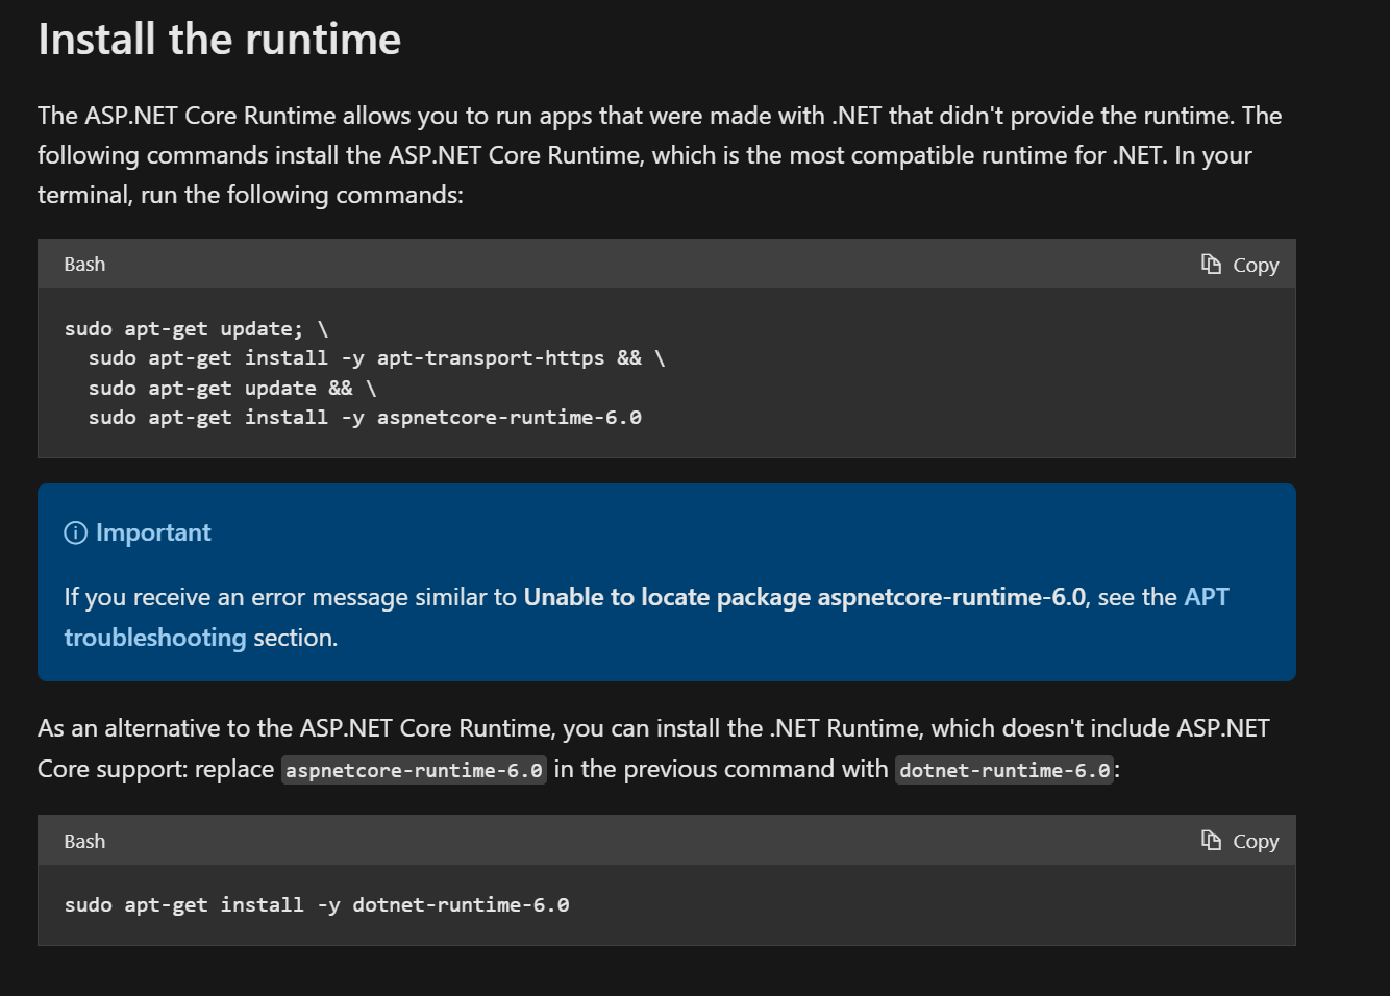
\includegraphics[width=1\textwidth]{img/03_2_runtime_documentation}
    ~\caption{Install the .NET SDK or the .NET Runtime on Ubuntu MSDN.}\label{fig:figure7}
\end{figure}
We install .NET runtime using the commands
\begin{itemize}
    \item \texttt{sudo apt-get update}
    \item \texttt{sudo apt-get install -y apt-transport-https}
    \item \texttt{sudo apt-get update}
    \item \texttt{sudo apt-get install -y aspnetcore-runtime-6.0}
\end{itemize}
Terminal output as follows
\begin{figure}[H]
    \centering
    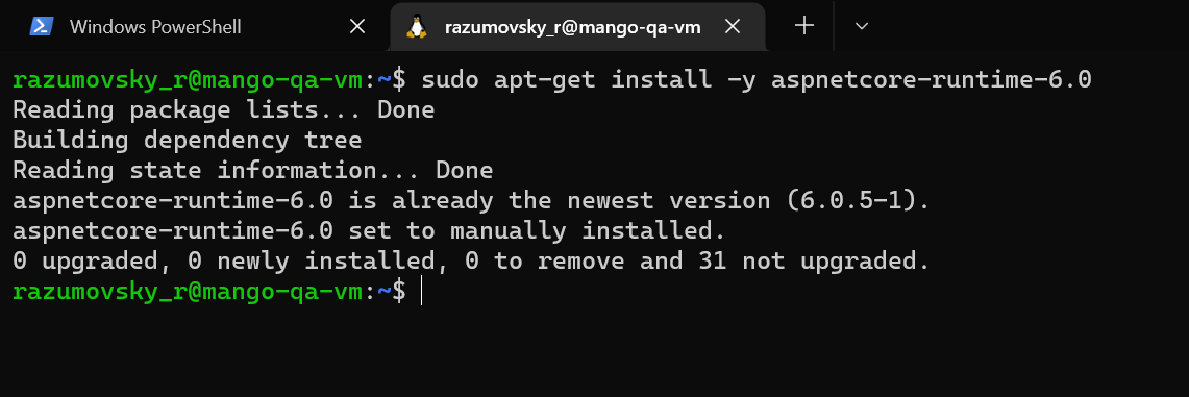
\includegraphics[width=1\textwidth]{img/03_6_runtime_install}
    ~\caption{Ubuntu 20.04 install .NET 6.0 Runtime terminal output.}\label{fig:figure8}
\end{figure}
Therefore, the .NET SDK and Runtime are installed so that we are able to run specified .NET app on behalf of
our Ubuntu virtual machine.



    \section{Copy build files to the VM via SSH}\label{sec:copy-build-files-to-the-vm-via-ssh}
    Now we have to build our .NET Core Web Application to the specified folder, say \texttt{/mango-linux-build/src}.
Note that it is much better to build it on behalf of Windows 10 main machine, not WSL 2.0 one.
We use the following commands to build .NET Core Web App with \texttt{Release} configuration
\begin{itemize}
    \item \texttt{cd E:/RiderProjects/MangoMessengerAPI/MangoAPI.Presentation}
    \item \texttt{dotnet publish "MangoAPI.Presentation.csproj" -r linux-x64 \\ -o /mango-linux-build/src}
\end{itemize}
Terminal output is as follows
\begin{figure}[H]
    \centering
    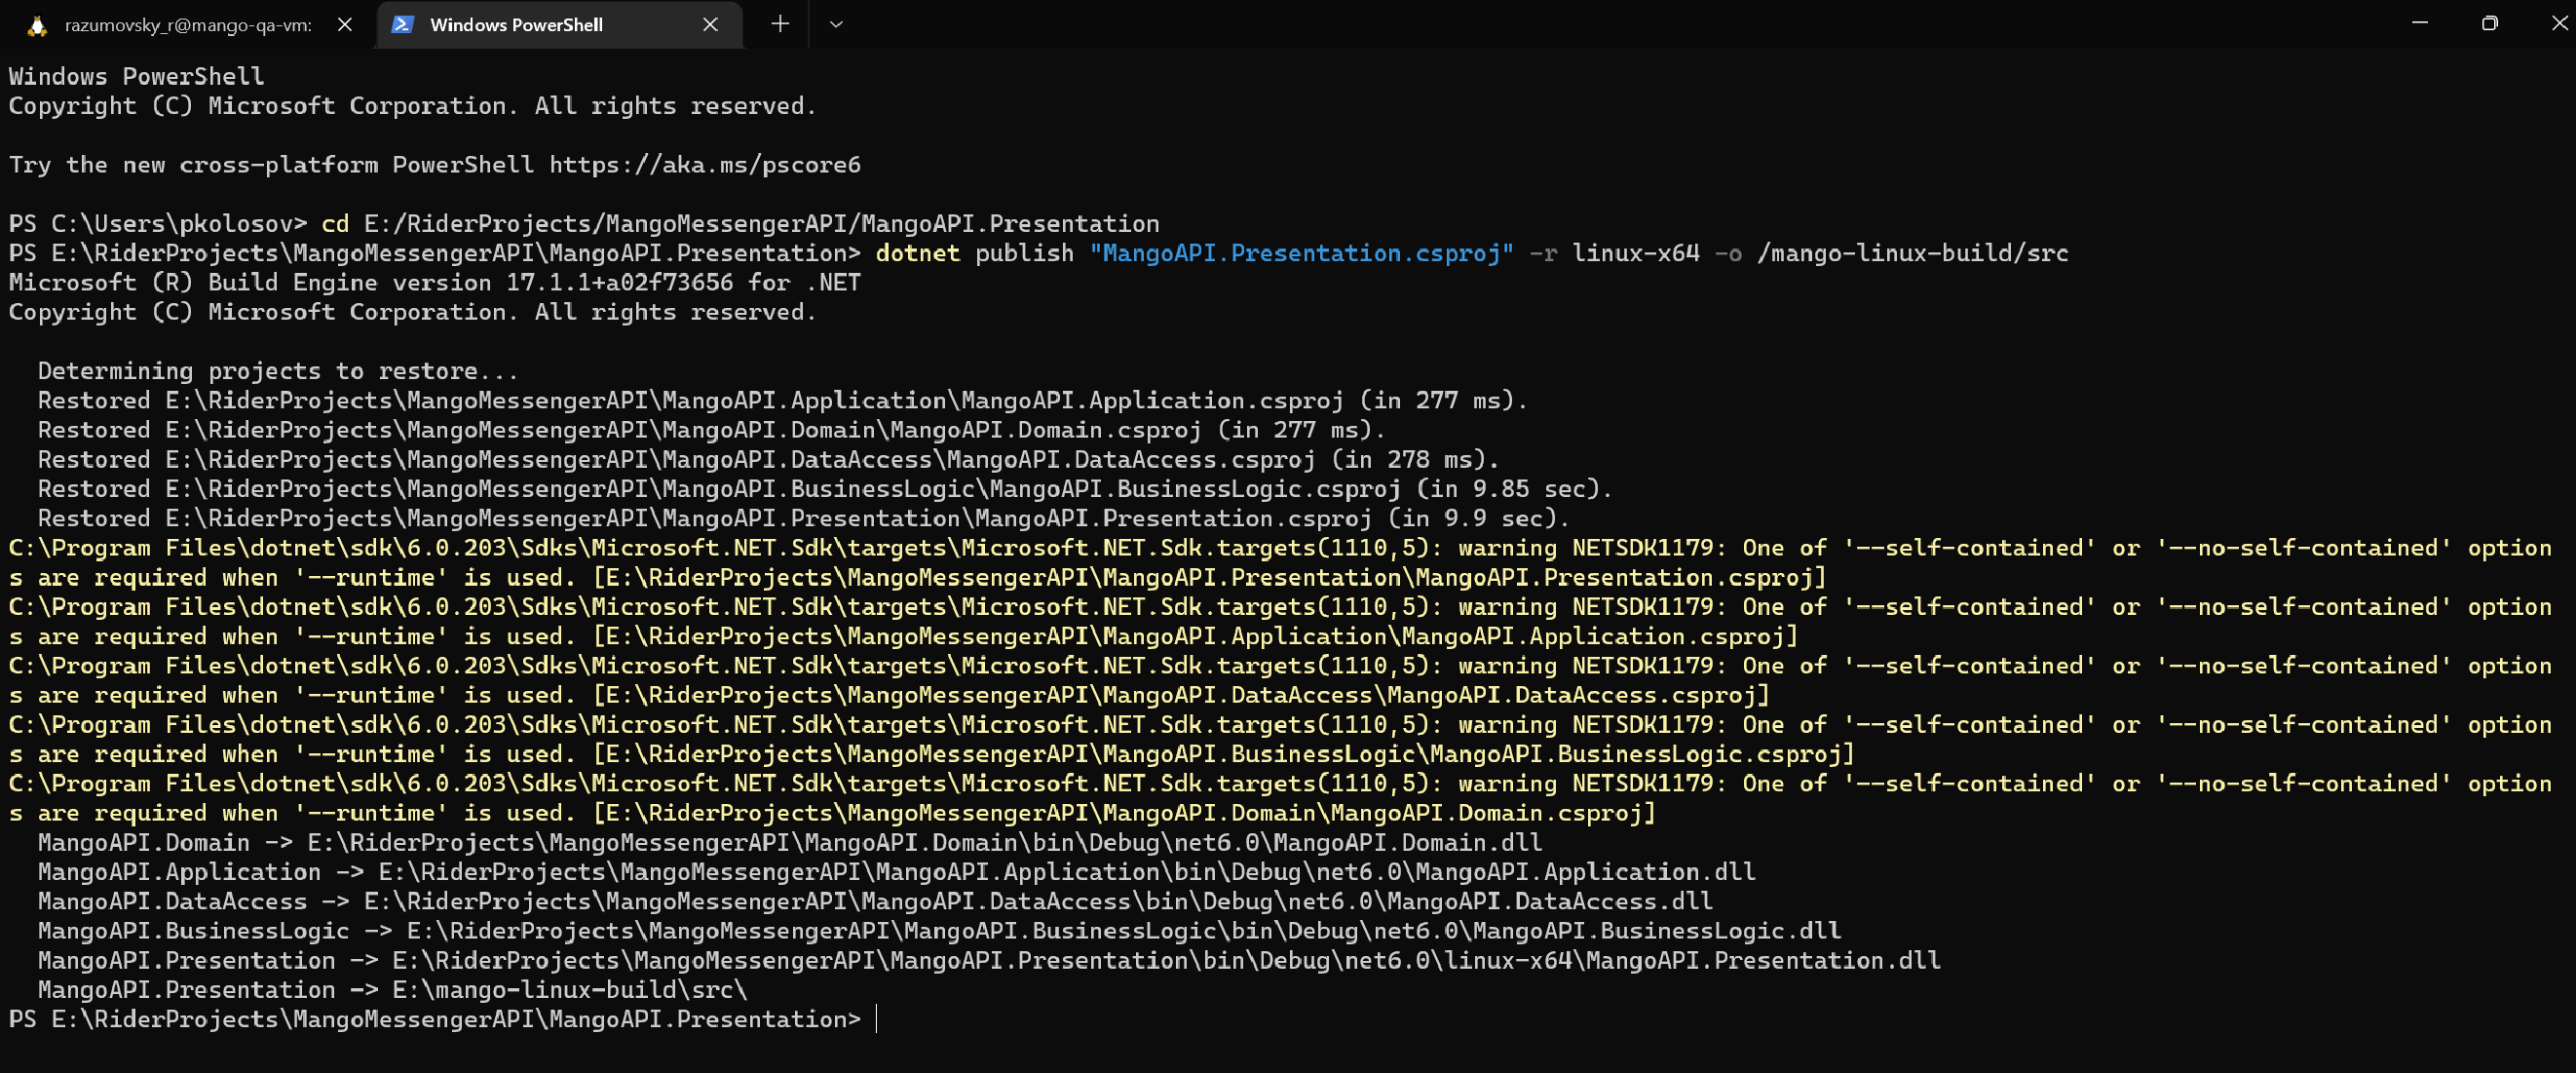
\includegraphics[width=1\textwidth]{img/04_build_application}
    ~\caption{Build .NET Web app terminal output.}\label{fig:figure9}
\end{figure}
Let's create the folder \texttt{mango-backend} where build files to be stored.
Do not forget to connect to your Azure VM via SSH\@.
Do not also forget to assign read-write privileges to the folder, using the commands
\begin{itemize}
    \item \texttt{sudo mkdir ~/mango-backend}
    \item \texttt{sudo chmod a+rwx ~/mango-backend}
\end{itemize}
Terminal output:
\begin{figure}[H]
    \centering
    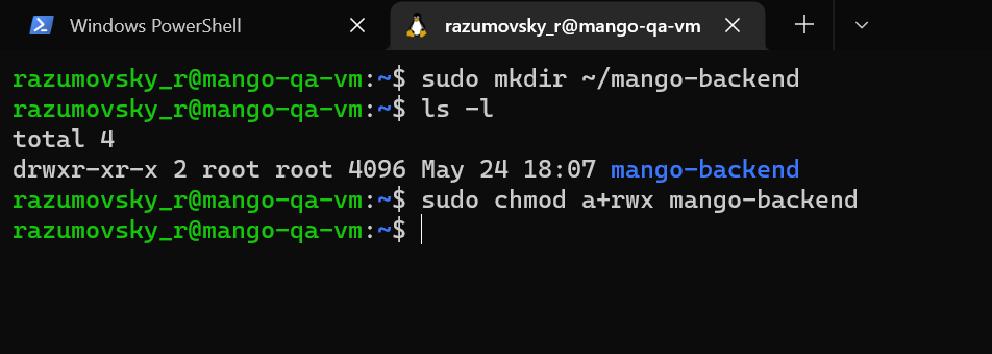
\includegraphics[width=1\textwidth]{img/04_create_remote_folder}
    ~\caption{Create folder at remote VM.}\label{fig:figure10}
\end{figure}
As next step consider to copy build files to the remote folder on your Azure VM so that we execute our program after.
We copy the build files on behalf of WSL2 this time.
In order to copy the build files we use following commands
\begin{itemize}
    \item \texttt{cd /mnt/e/mango-linux-build}
    \item \texttt{scp -r -i ~/.ssh/id\_rsa ./src/* \\ razumovsky\_r@VM\_IP\_ADDRESS:/home/razumovsky\_r/mango-backend}
\end{itemize}
where \texttt{id\_rsa} is the private key.
Terminal output:
\begin{figure}[H]
    \centering
    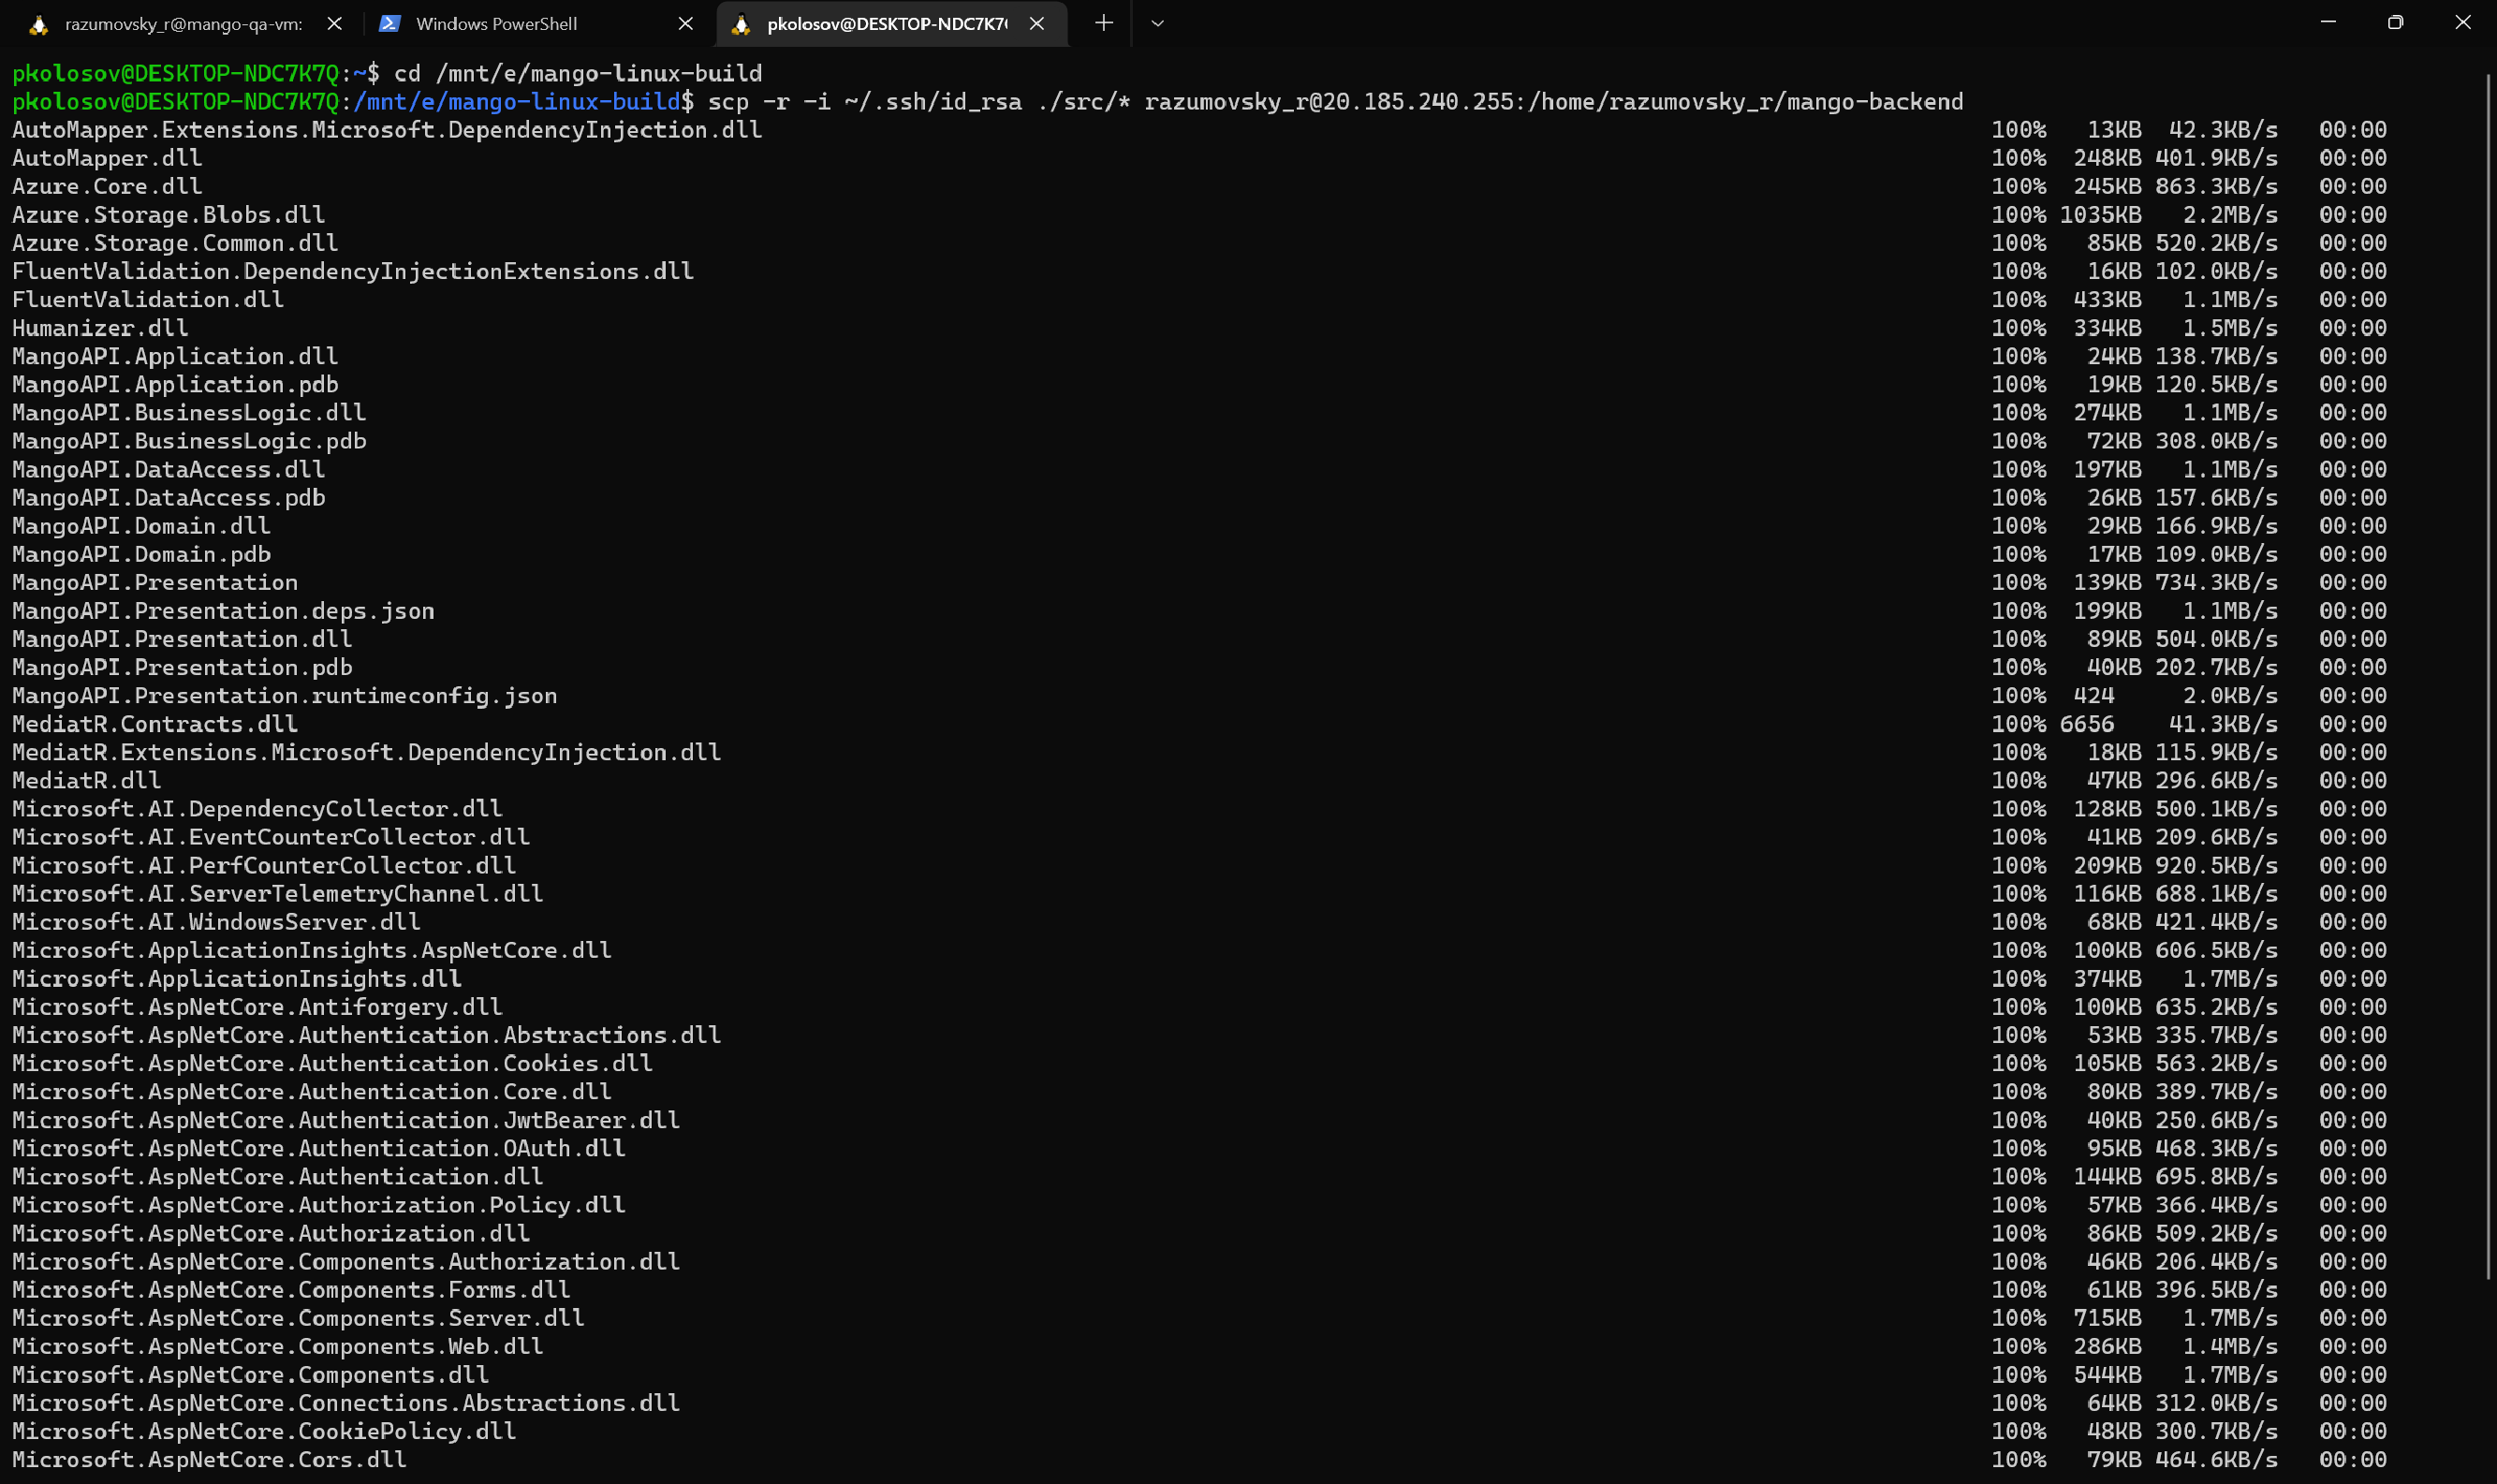
\includegraphics[width=1\textwidth]{img/04_copy_build_files_via_ssh}
    ~\caption{Copy build files via SSH.}\label{fig:figure11}
\end{figure}
Ensure build files are copied successfully to the remote VM, use the command \texttt{ls -l mango-backend}.
Terminal output:
\begin{figure}[H]
    \centering
    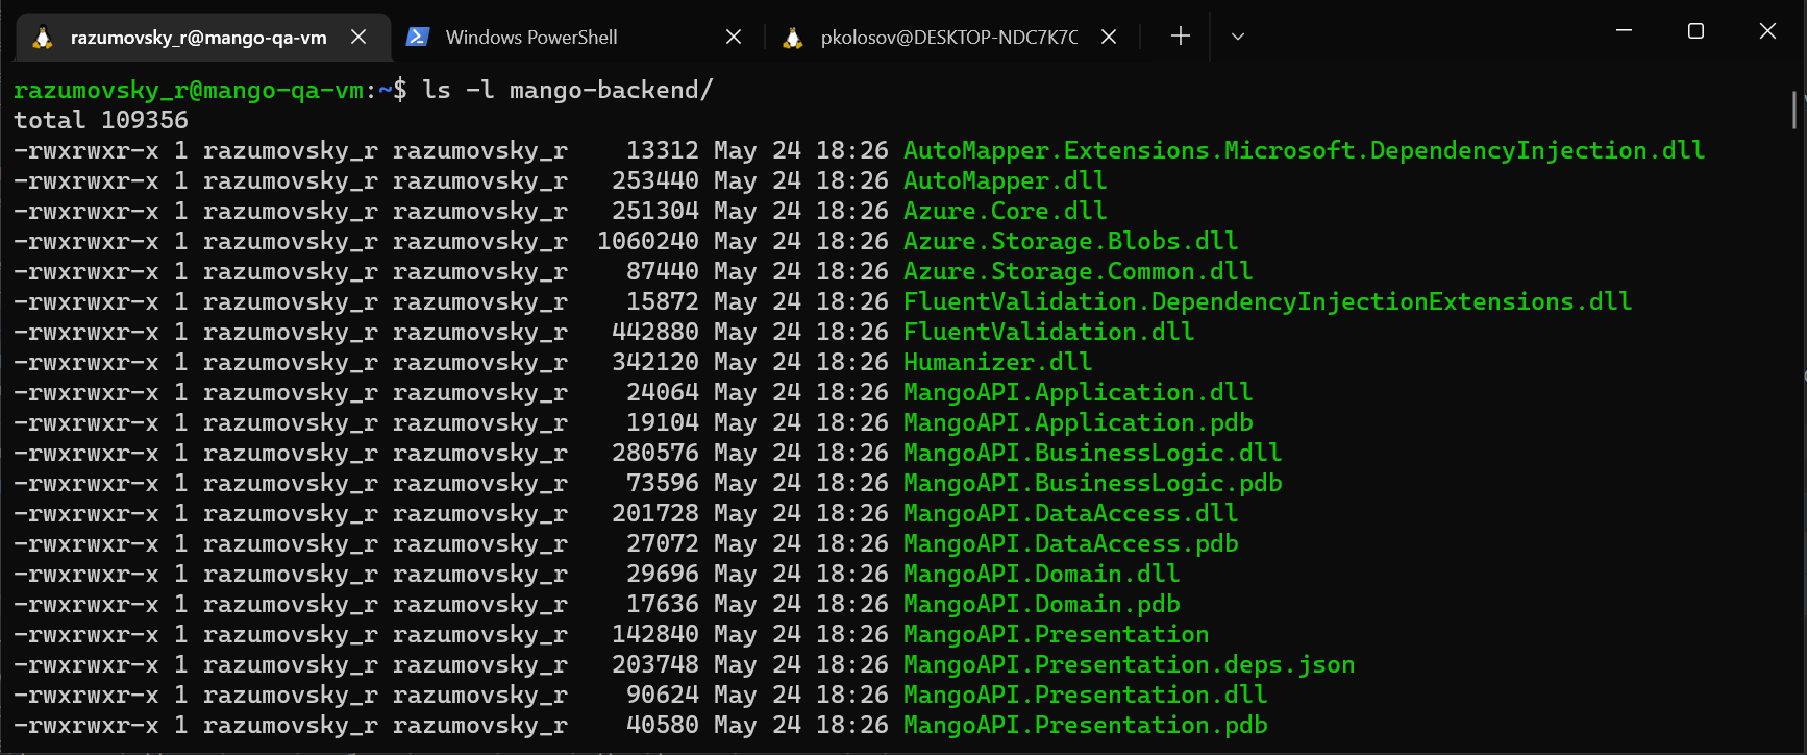
\includegraphics[width=1\textwidth]{img/04_verify_files_on_remote_vm}
    ~\caption{Check files at remote VM.}\label{fig:figure12}
\end{figure}




    \section{Configure Ubuntu service}\label{sec:configure-ubuntu-service}
    In this section the main aim is to implement an Ubuntu service such that runs our previously built
.NET Core web application.
It means that we have to configure the environment variables used in our application
as well as to configure the firewall rules so that application will be able to communicate with
another resources like databases, blobs etc.
Ubuntu server refers to the entry point of the web app, that is
\begin{center}
    \texttt{/home/razumovsky\_r/mango-backend/MangoAPI.Presentation}
\end{center}
Use the command to create service
\begin{center}
    \texttt{sudo vim /etc/systemd/system/mangoback.service}
\end{center}
Paste the following text there
\begin{spverbatim}
[Unit]
    Description=Mango Messenger Backend Service for Azure Dev Environment
    After=network.target

    [Service]
    Environment=ASPNETCORE_URLS=http://+:8080/
    Environment=MANGO_JW_ISSUER="https://front.mangomessenger.company"
    Environment=MANGO_JWT_AUDIENCE="https://back.mangomessenger.company"
    Environment=MANGO_JWT_SIGN_KEY="d32d7cea-4cb8-4488-aa94-323ffb8cbdf4"
    Environment=MANGO_EMAIL_NOTIFICATIONS_ADDRESS="mango@gmail.com"
    Environment=MANGO_FRONTEND_ADDRESS="https://front.mangomessenger.company/"
    Environment=MANGO_DATABASE_URL="database.connection.string"
    Environment=MANGO_SEED_PASSWORD="seedPass"
    Environment=MANGO_BLOB_URL="blob.url.connection.string"
    Environment=MANGO_BLOB_CONTAINER="container.name"
    Environment=MANGO_BLOB_ACCESS="blob.access.url"
    Environment=MANGO_MAILGUN_API_KEY="mailgun.api.key"
    Environment=MANGO_MAILGUN_API_BASE_URL="https://api.mailgun.net"
    Environment=MANGO_MAILGUN_API_BASE_DOMAIN="back.mangomessenger.company"
    Environment=MANGO_BACKEND_ADDRESS="https://back.mangomessenger.company/"
    Type=simple
    WorkingDirectory=/home/razumovsky_r/mango-backend
    ExecStart=/home/razumovsky_r/mango-backend/MangoAPI.Presentation
    User=razumovsky_r
    Group=razumovsky_r

    [Install]
    WantedBy=multi-user.target
\end{spverbatim}
From the vim it should look as follows
\begin{figure}[H]
    \centering
    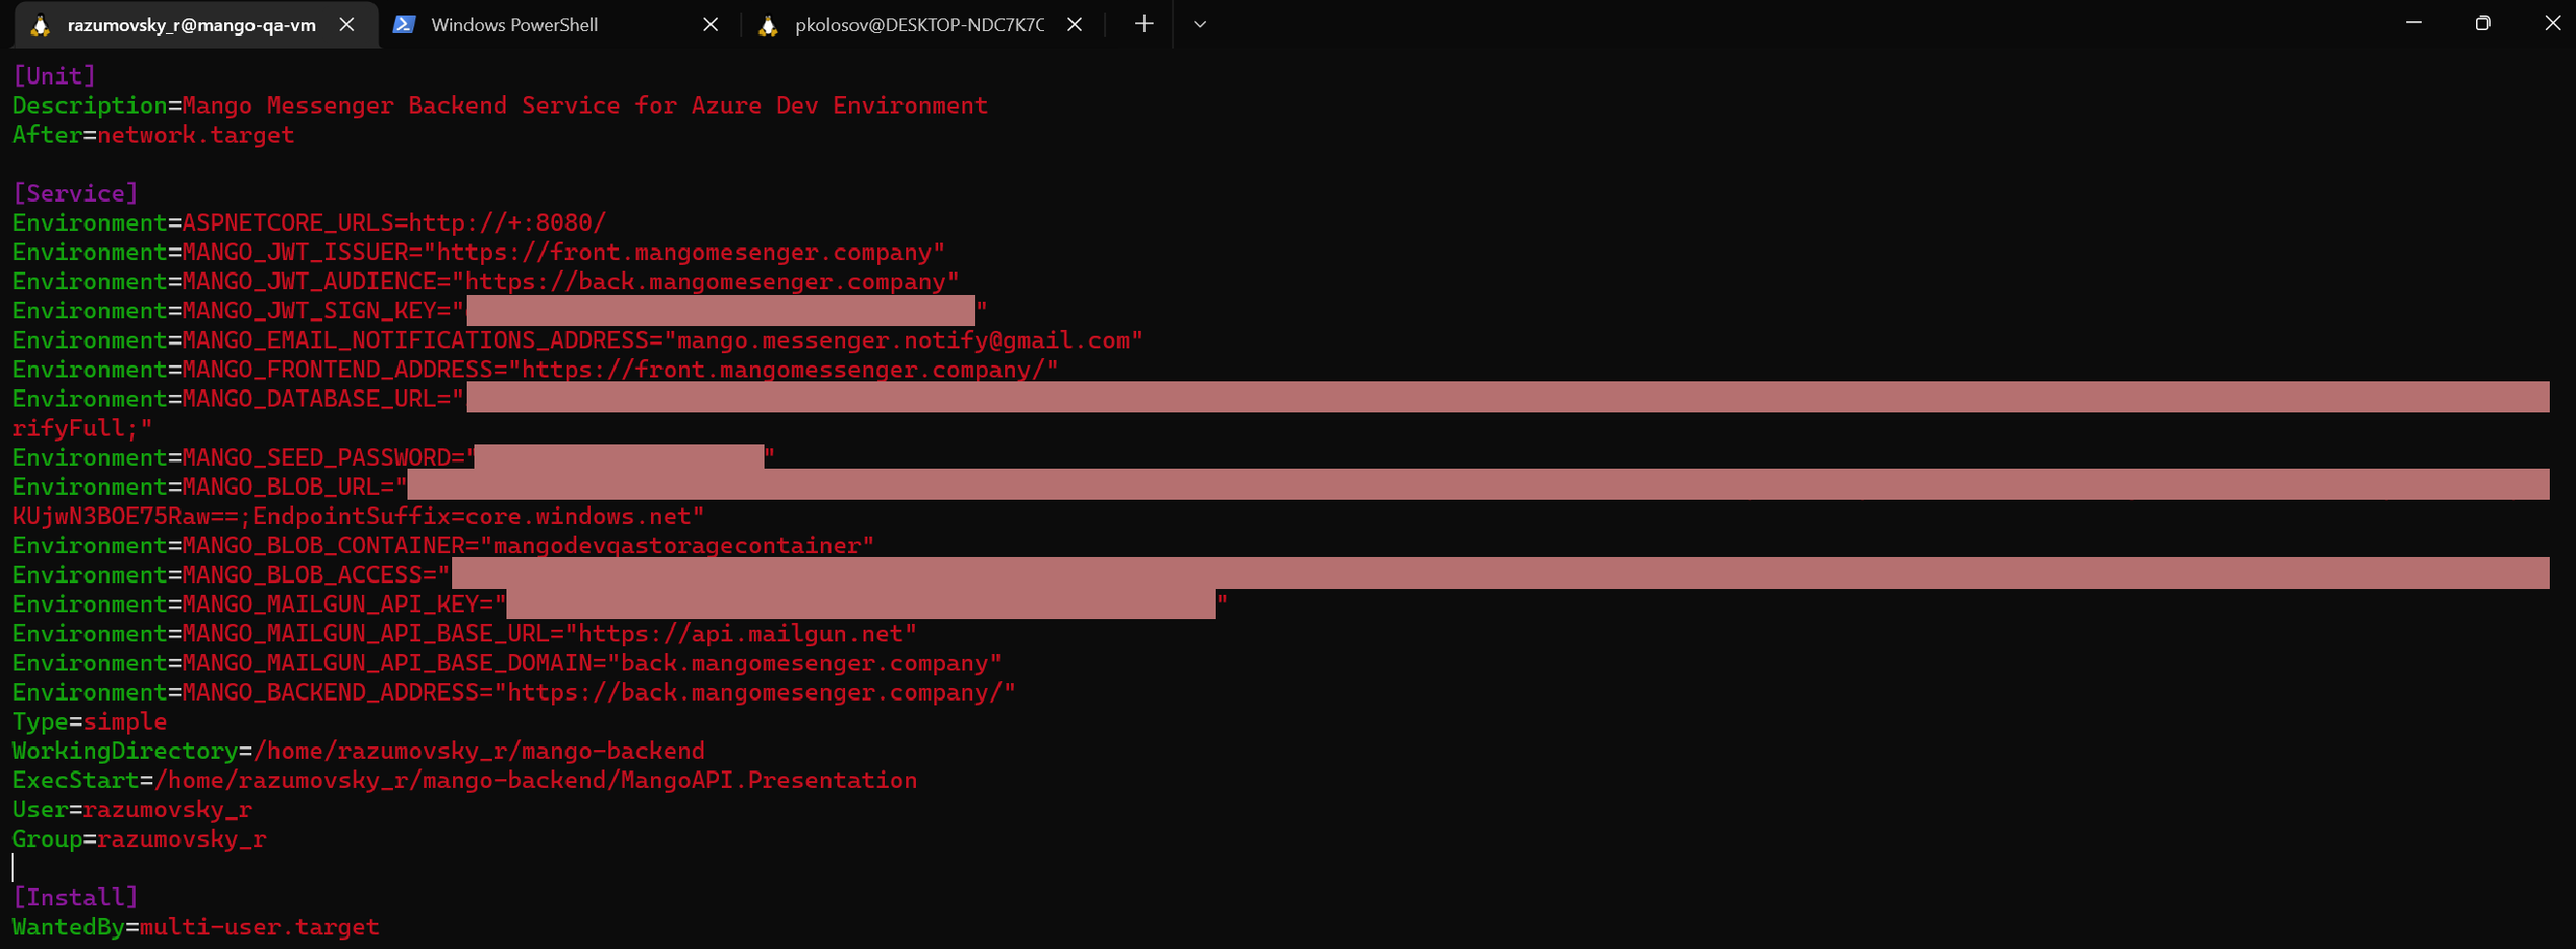
\includegraphics[width=1\textwidth]{img/05_ubuntu_service_vim}
    ~\caption{Ubuntu service opened in vim.}\label{fig:figure13}
\end{figure}
Make sure all resources are listening from the outside, check firewall rules on database side prior to run the service.
Start and check health of the service using
\begin{itemize}
    \item \texttt{sudo systemctl start mangoback}
    \item \texttt{sudo systemctl status mangoback}
\end{itemize}
Terminal output:
\begin{figure}[H]
    \centering
    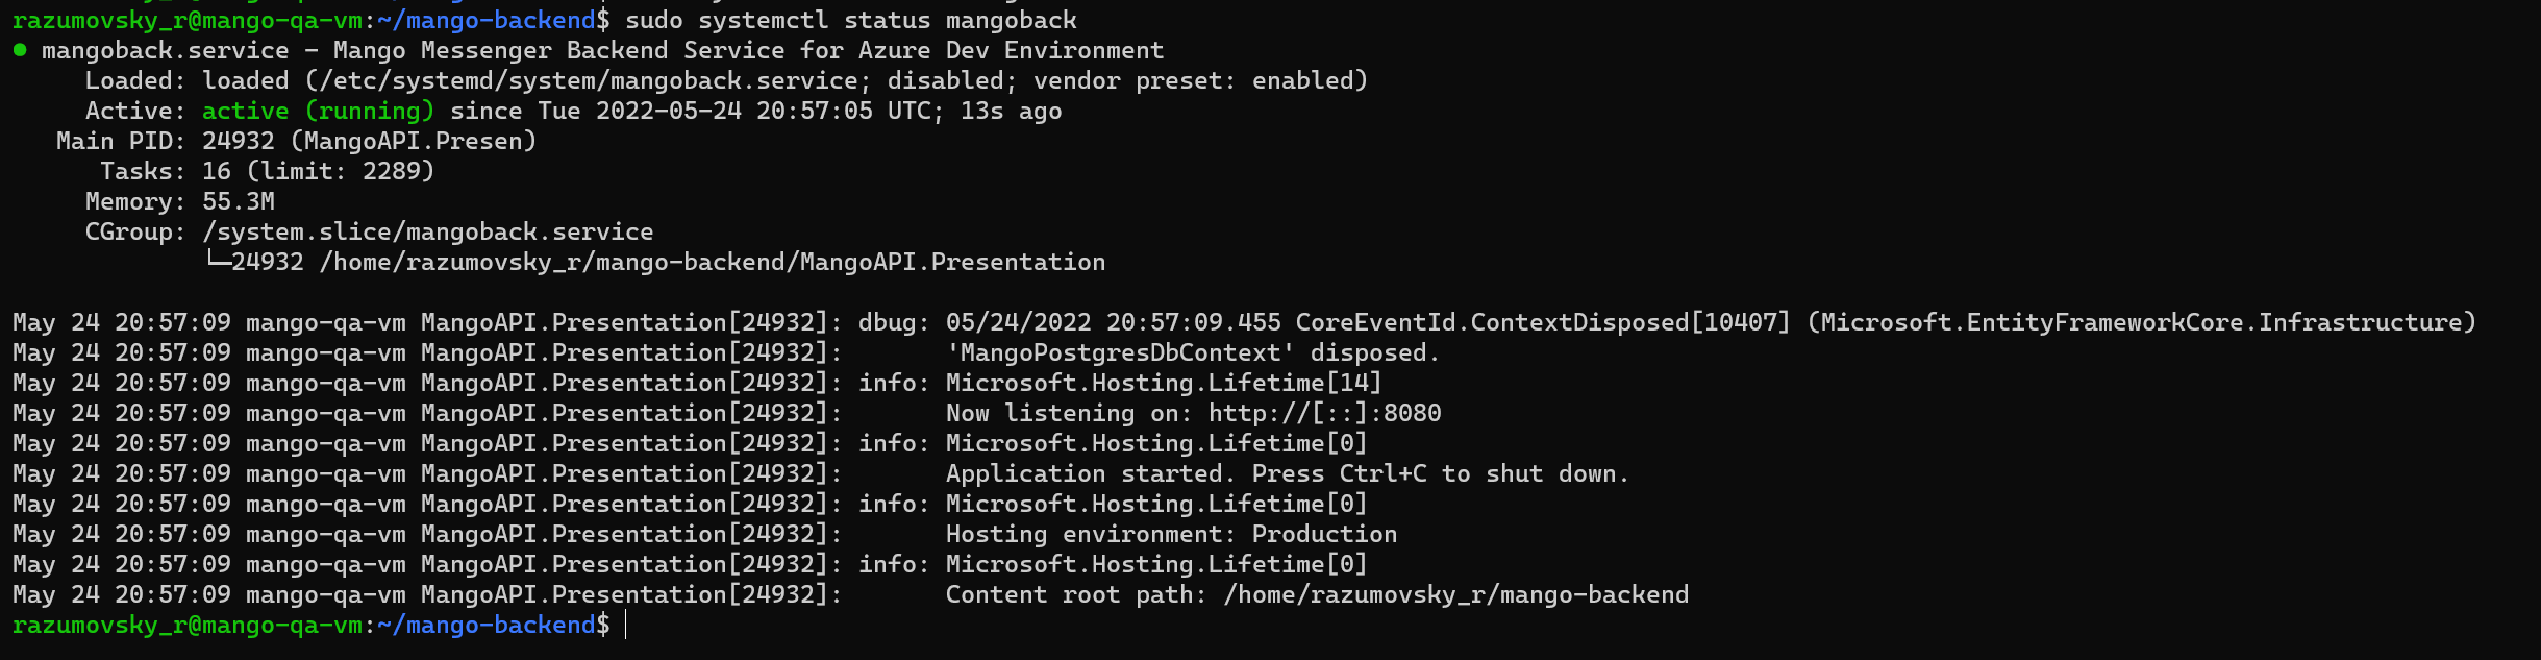
\includegraphics[width=1\textwidth]{img/05_ubuntu_service_status}
    ~\caption{Run ubuntu service and check status, terminal output.}\label{fig:figure14}
\end{figure}
This completes the section.



    \section{Install and configure Nginx server}\label{sec:install-and-configure-nginx-server}
    Now we have to configure the \texttt{nginx} server in order to expose our .NET Core web application to the outside.
As a result of this section web app will be exposed and accessible via VM's external IP address.
Let's install it using the commands
\begin{itemize}
    \item \texttt{sudo apt update -y}
    \item \texttt{sudo apt install -y nginx build-essential}
\end{itemize}
Terminal output:
\begin{figure}[H]
    \centering
    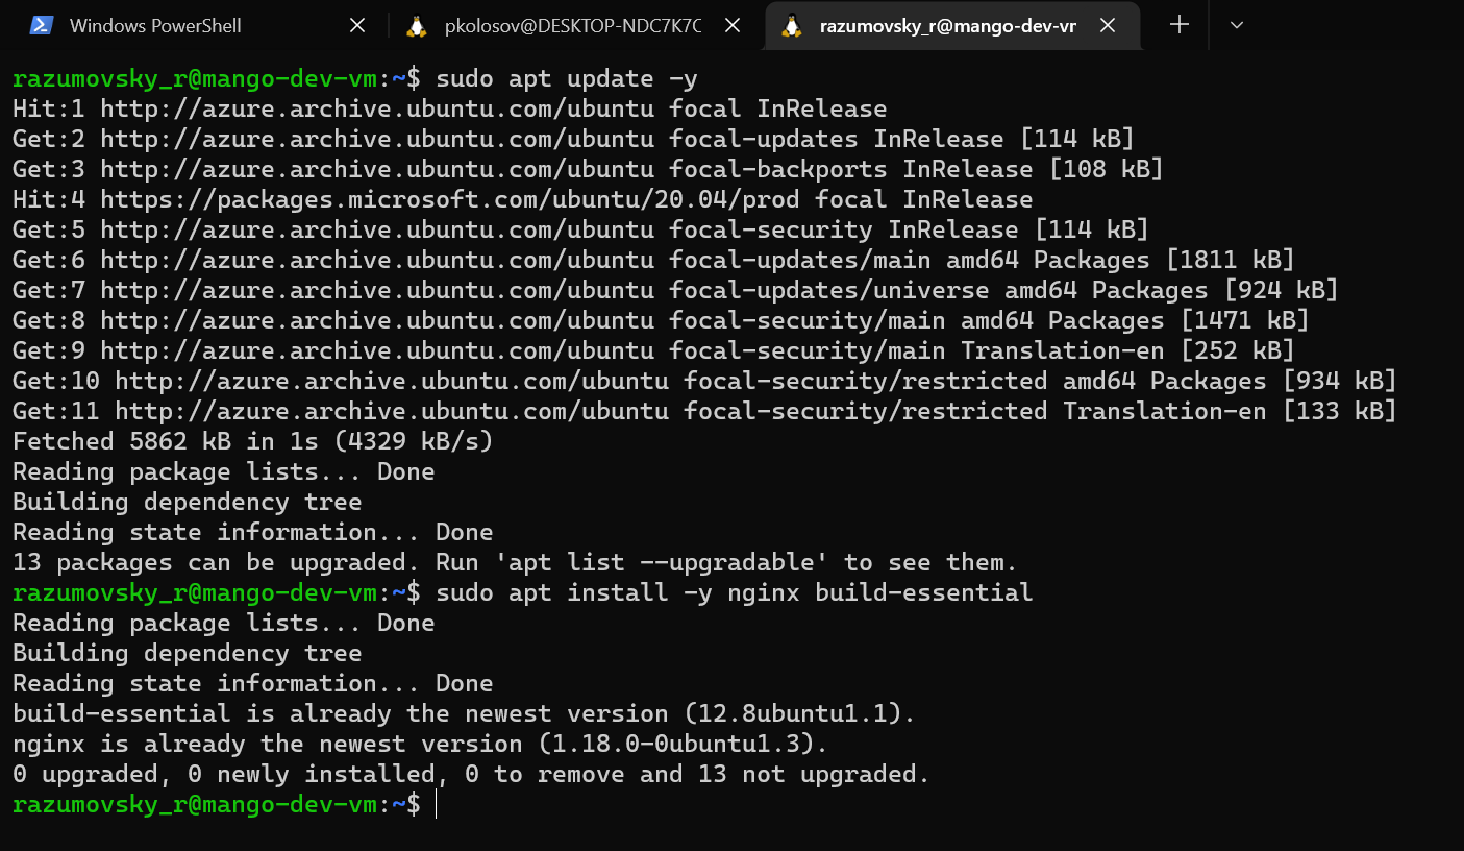
\includegraphics[width=1\textwidth]{img/06_install_nginx}
    ~\caption{Ubuntu install nginx terminal output.}\label{fig:figure15}
\end{figure}
Next, it is necessary to create nginx configuration that exposes our application, that is
\begin{spverbatim}
    server {
        server_name STATIC_IP_ADDRESS_OF_VM;

        location / {
            include proxy_params;
            proxy_pass http://127.0.0.1:8080;
        }

        location /swagger {
            include proxy_params;
            proxy_pass http://127.0.0.1:8080;
        }

        location /api {
            include proxy_params;
            proxy_pass http://127.0.0.1:8080;
        }

        location /notify {
            proxy_pass http://127.0.0.1:8080;
            proxy_http_version 1.1;
            proxy_set_header Upgrade $http_upgrade;
            proxy_set_header Connection "upgrade";
            proxy_set_header Host $host;
            proxy_cache_bypass $http_upgrade;
        }
    }
\end{spverbatim}
We create it at the following path on behalf of our Azure VM via SSH
\begin{center}
    \texttt{sudo vim /etc/nginx/conf.d/back.mangomesenger.company.conf}
\end{center}
Restart nginx and validate its state using the commands
\begin{itemize}
    \item \texttt{sudo systemctl restart nginx}
    \item \texttt{sudo nginx -t}
\end{itemize}
Terminal output:
\begin{figure}[H]
    \centering
    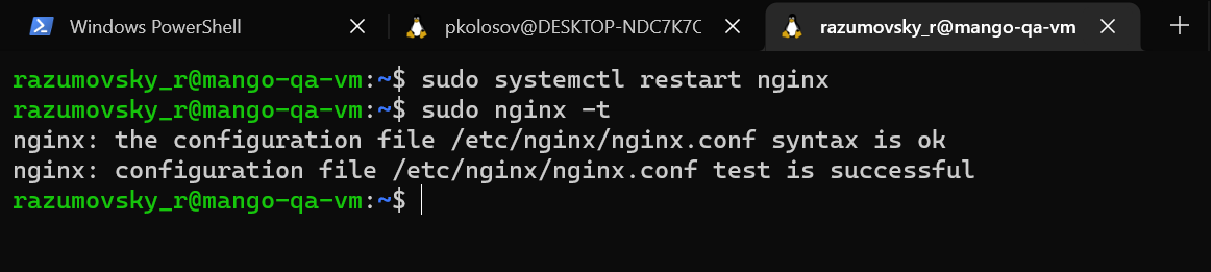
\includegraphics[width=1\textwidth]{img/06_test_nginx}
    ~\caption{Restart and test nginx terminal output.}\label{fig:figure16}
\end{figure}
Now we must be able to find our application listening to the
\begin{center}
    \texttt{http://STATIC\_IP\_ADDRESS\_OF\_THE\_VM}
\end{center}
And actually it works as expected
\begin{figure}[H]
    \centering
    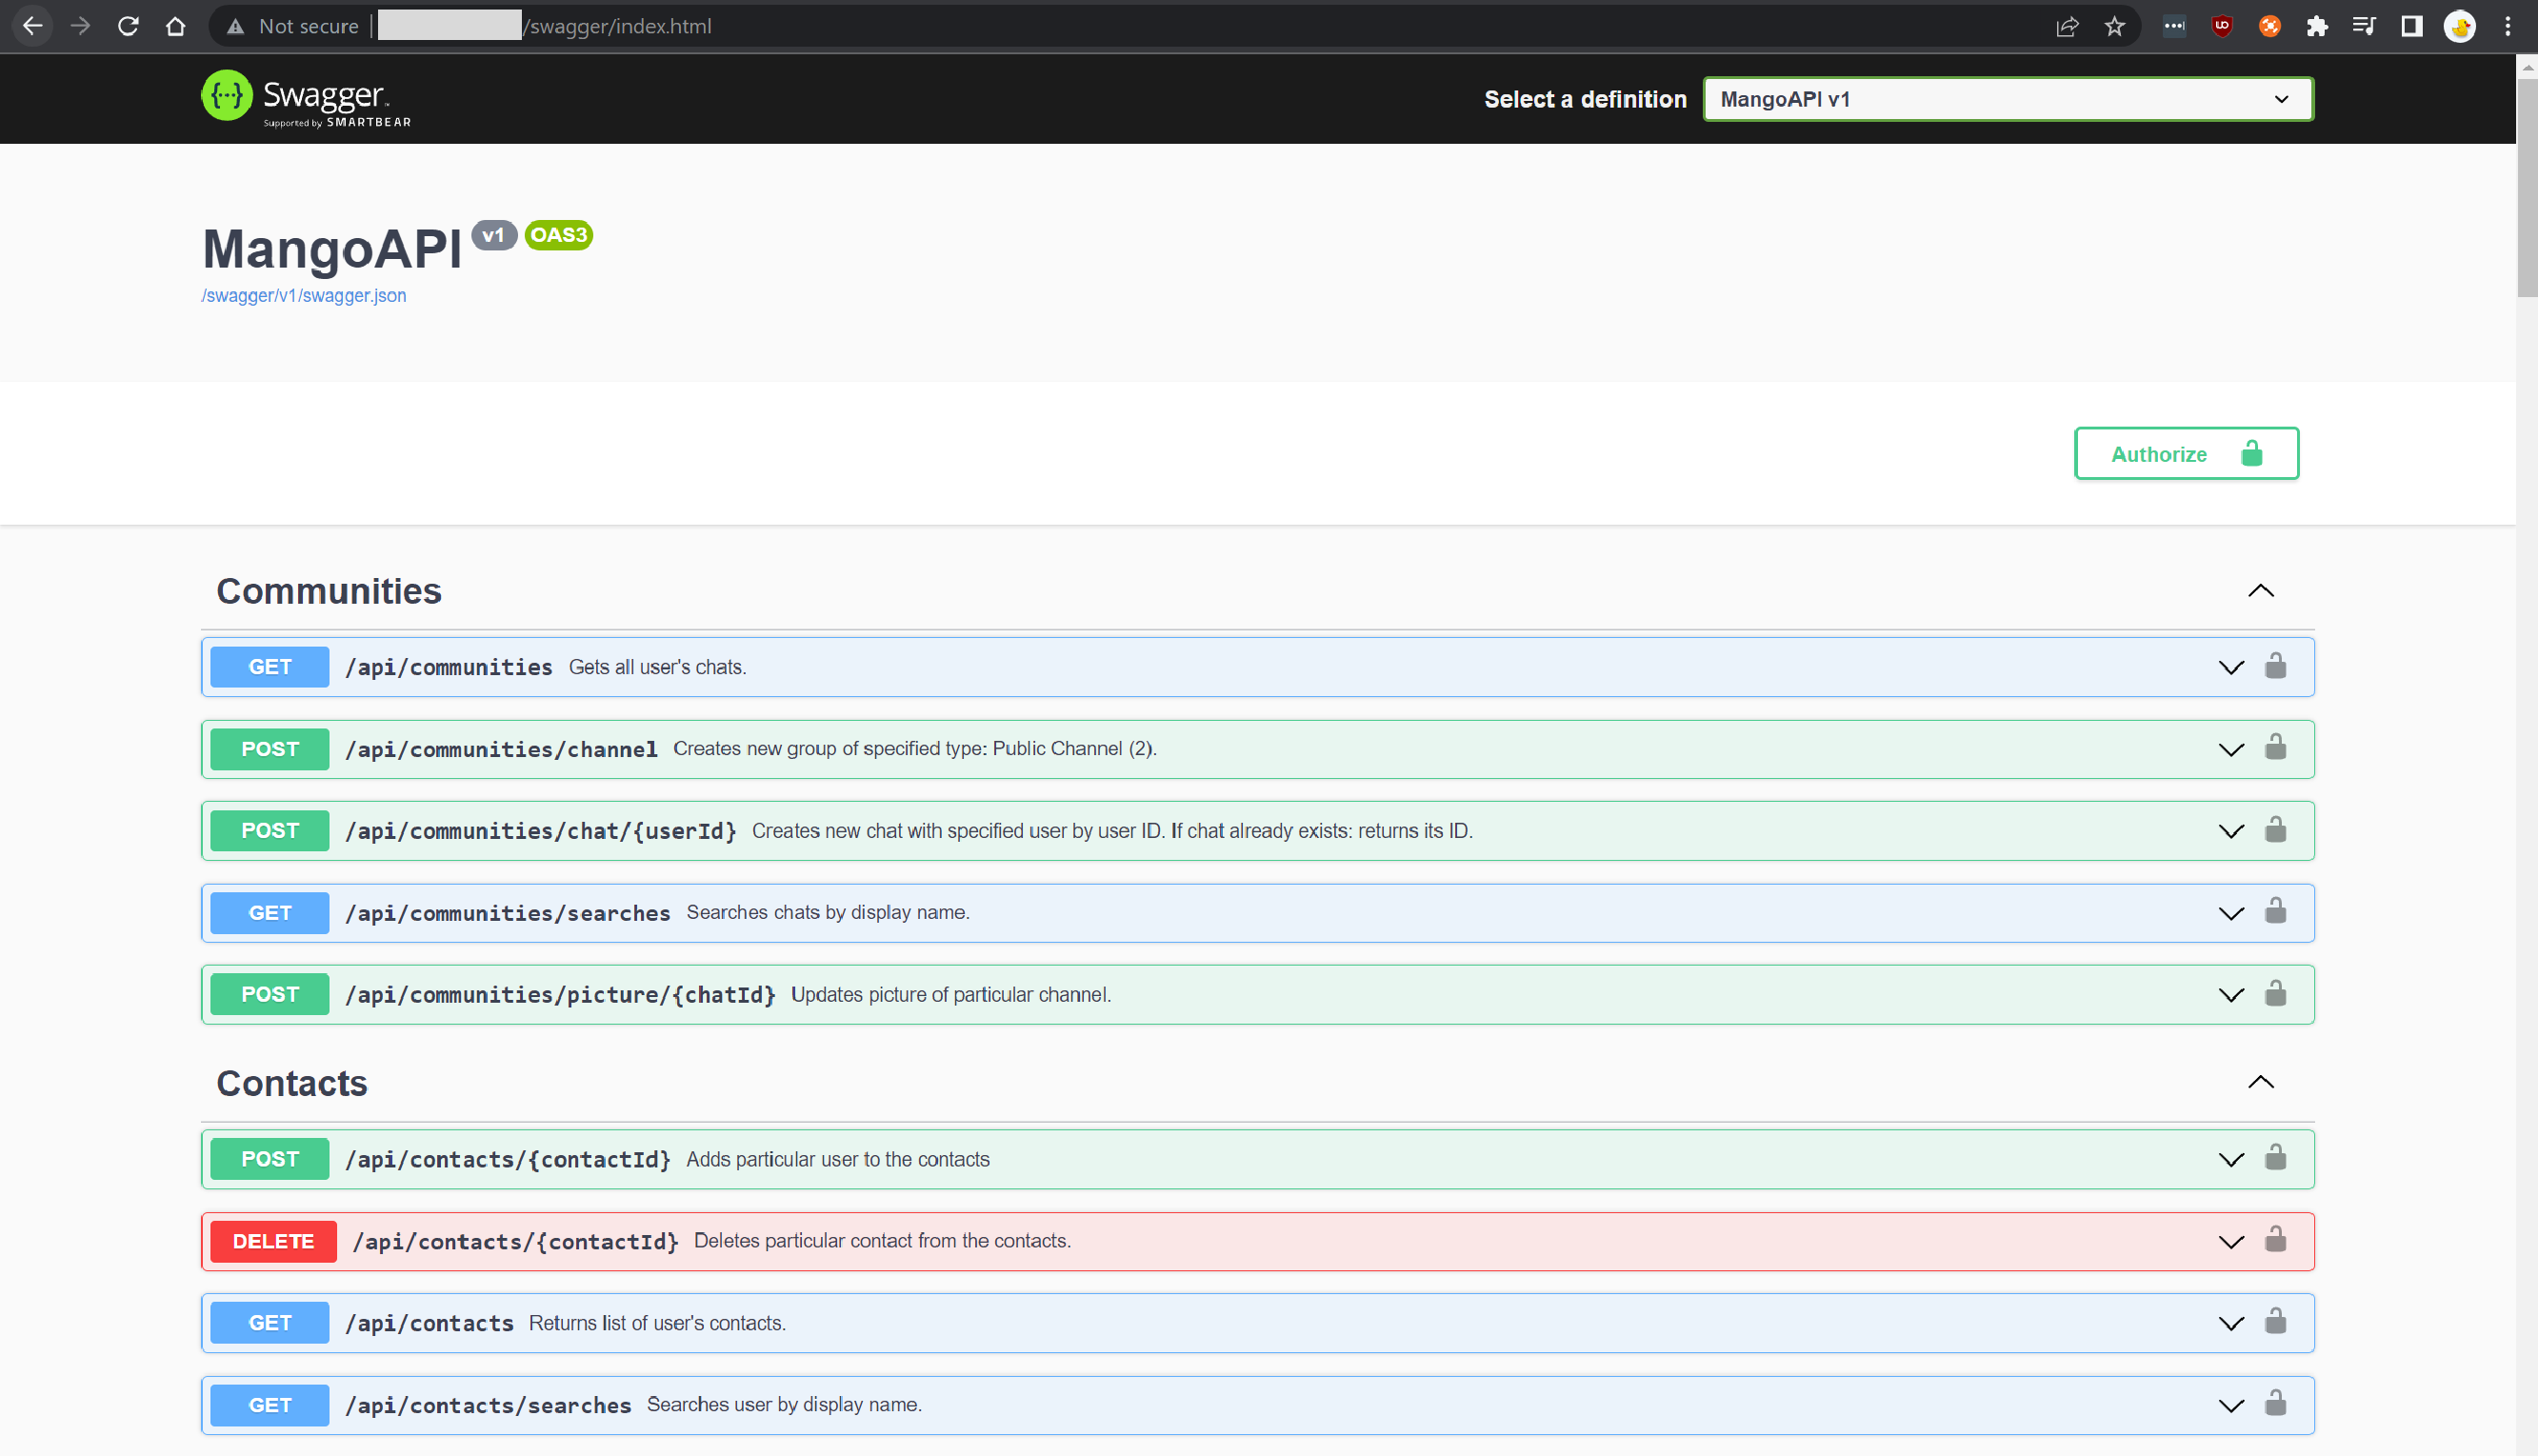
\includegraphics[width=1\textwidth]{img/06_view_in_browser}
    ~\caption{.NET Core web app accessed via browser using static IP address of the virtual machine.}\label{fig:figure17}
\end{figure}



    \section{Configure domain name and SSL}\label{sec:configure-domain-name-and-ssl}
    In this section our main aim is to assign specified (previously bought) domain name to our .NET Core web application
as well as to configure SSL certificate for it.
What is domain name's definition?
\begin{center}
    \textbf{Domain name} -- is a string of text that maps to a numeric IP address, used to access a website
    from client software~\cite{DomanNameCloudflare}.
    The actual address of a website is a complex numerical IP address (e.g.\ 103.21.244.0), but thanks to DNS,
    users are able to enter human-friendly domain names and be routed to the websites they are looking for.
\end{center}

\subsection{Buy and configure domain name using Cloudflare}\label{subsec:buy-and-configure-domain-name-using-cloudflare}
For instance, the domain name can be bought on the one of the following resources
\begin{itemize}
    \item \href{https://www.name.com/}{\texttt{https://www.name.com}}
    \item \href{https://www.namecheap.com/}{\texttt{https://www.namecheap.com}}
    \item \href{https://get.tech/}{\texttt{https://get.tech}}
\end{itemize}
After that we have to associate our domain with the \href{https://www.cloudflare.com/}{\texttt{cloudflare.com}} service in order
to manage out domain name and get some free DDoS protection and request analytics.
For instance, I have bought a domain name withing \href{https://www.name.com/}{\texttt{name.com}} service
and configured it using the following DNS records:
\begin{itemize}
    \item \texttt{hassan.ns.cloudflare.com}
    \item \texttt{sonia.ns.cloudflare.com}
\end{itemize}
So it looks like as follows
\begin{figure}[H]
    \centering
    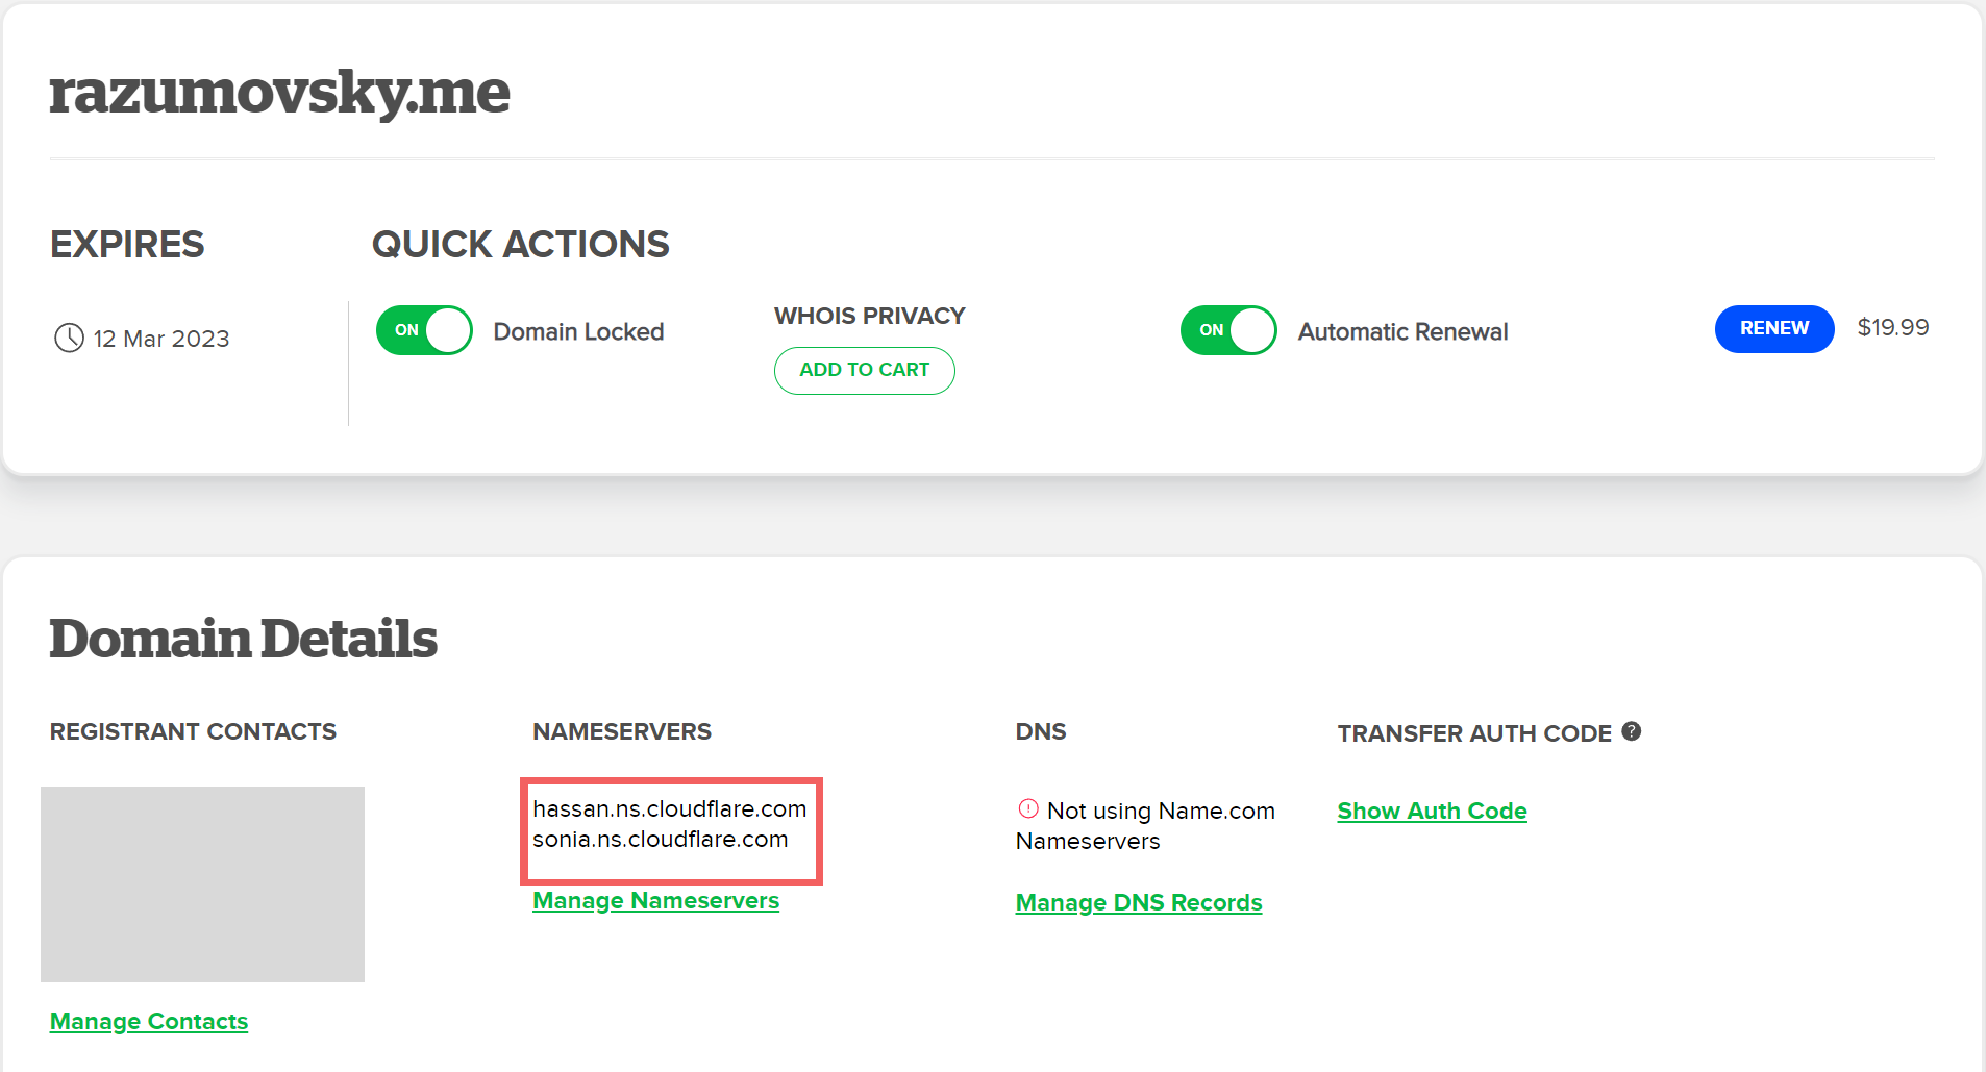
\includegraphics[width=1\textwidth]{img/07_domain_at_name_com}
    ~\caption{Domain name configuration at \href{https://www.name.com/}{\texttt{name.com}}.}\label{fig:figure18}
\end{figure}
After that we have to configure our domain name at cloudflare providing an IP address of the virtual machine we host
our .NET Core web application, that is
\begin{figure}[H]
    \centering
    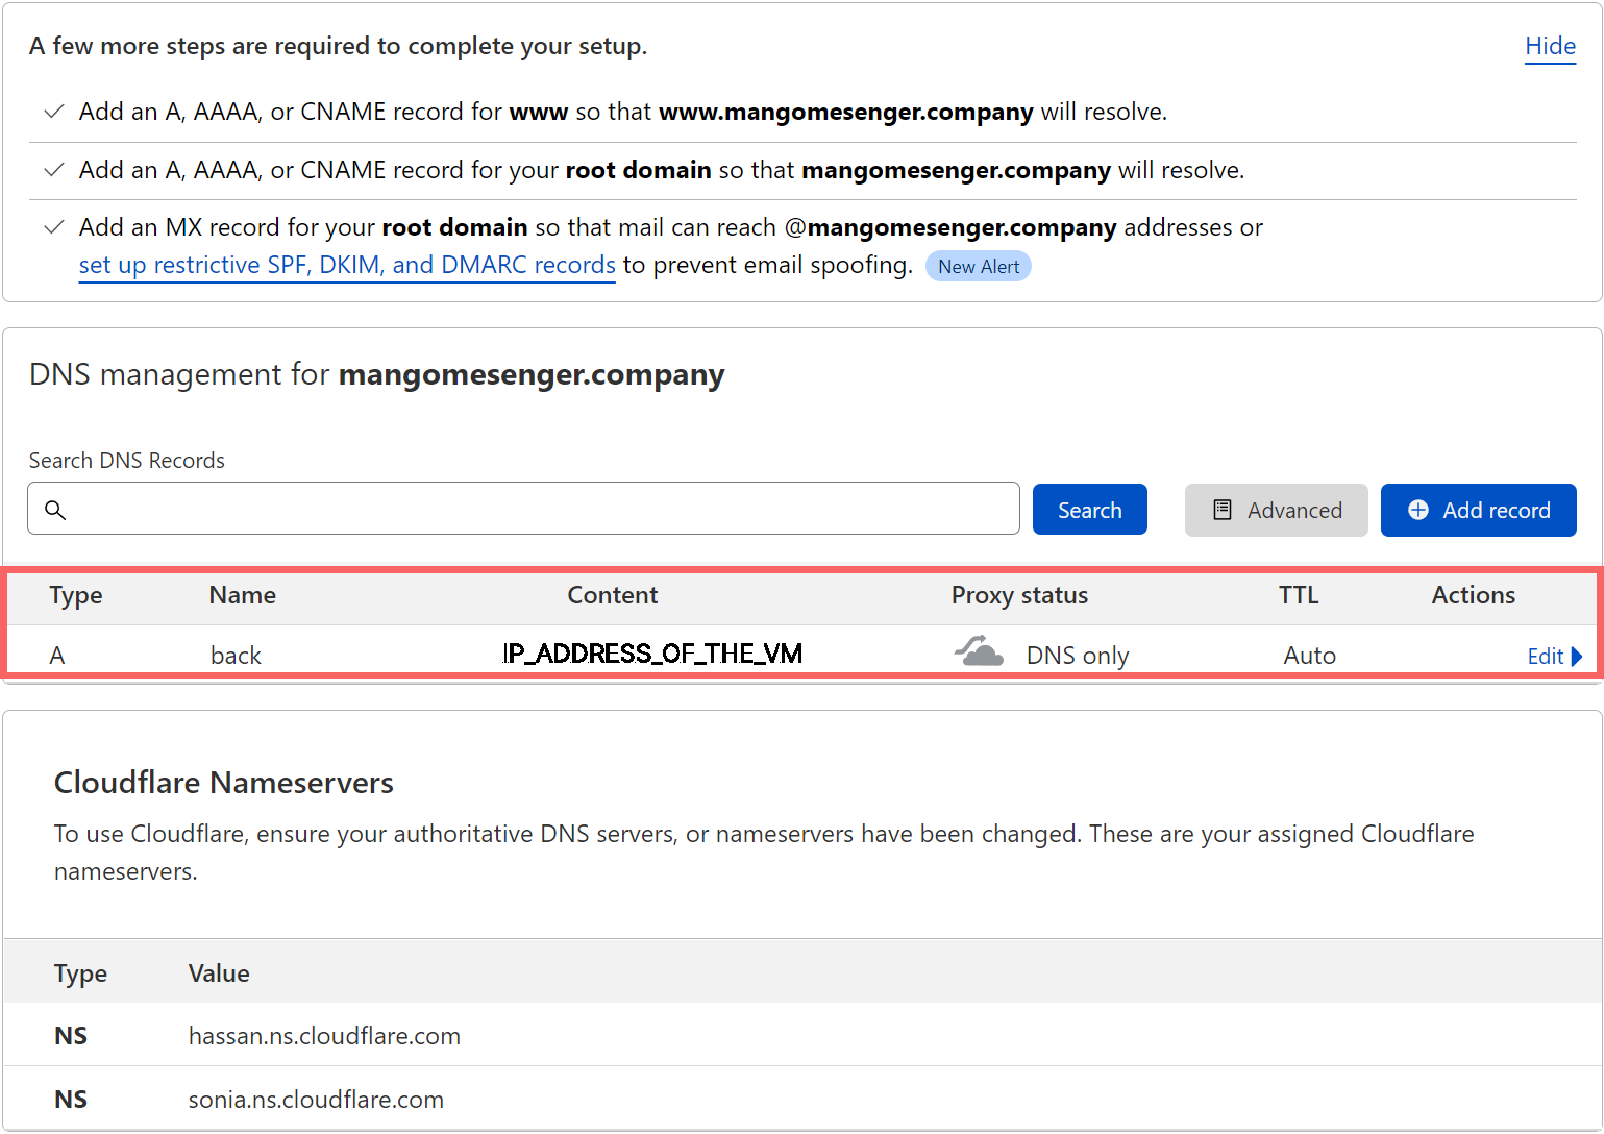
\includegraphics[width=1\textwidth]{img/07_domain_at_cloudflare_com}
    ~\caption{Domain name configuration at \href{https://www.cloudflare.com/}{\texttt{cloudflare.com}}.}\label{fig:figure19}
\end{figure}

\subsection{Configure nginx for the Domain name}\label{subsec:configure-nginx-for-the-domain-name}
Now our aim is to make sure that \texttt{nginx} server accepts connections to the VM via the Domain name we
previously bought and configured.
Yet again we use SSH + RSA key pair and change the address in our \texttt{nginx} configuration as follows
\begin{spverbatim}
    server {
        server_name back.mangomesenger.company;

        location / {
            include proxy_params;
            proxy_pass http://127.0.0.1:8080;
        }

        location /swagger {
            include proxy_params;
            proxy_pass http://127.0.0.1:8080;
        }

        location /api {
            include proxy_params;
            proxy_pass http://127.0.0.1:8080;
        }

        location /notify {
            proxy_pass http://127.0.0.1:8080;
            proxy_http_version 1.1;
            proxy_set_header Upgrade $http_upgrade;
            proxy_set_header Connection "upgrade";
            proxy_set_header Host $host;
            proxy_cache_bypass $http_upgrade;
        }
    }
\end{spverbatim}
We, actually, have changed only the top line \texttt{server\_name} to the
\begin{center}
    \texttt{server\_name back.mangomesenger.company;}
\end{center}
Let's restart and test the \texttt{nginx} server using the commands
\begin{itemize}
    \item \texttt{sudo systemctl restart nginx}
    \item \texttt{sudo nginx -t}
\end{itemize}
So that our web application is available now under the \texttt{HTTP} external url, yet without SSL certificate
\begin{center}
    \href{http://back.mangomesenger.company/swagger}{\texttt{http://back.mangomesenger.company/swagger}}
\end{center}
And it works as desired
\begin{figure}[H]
    \centering
    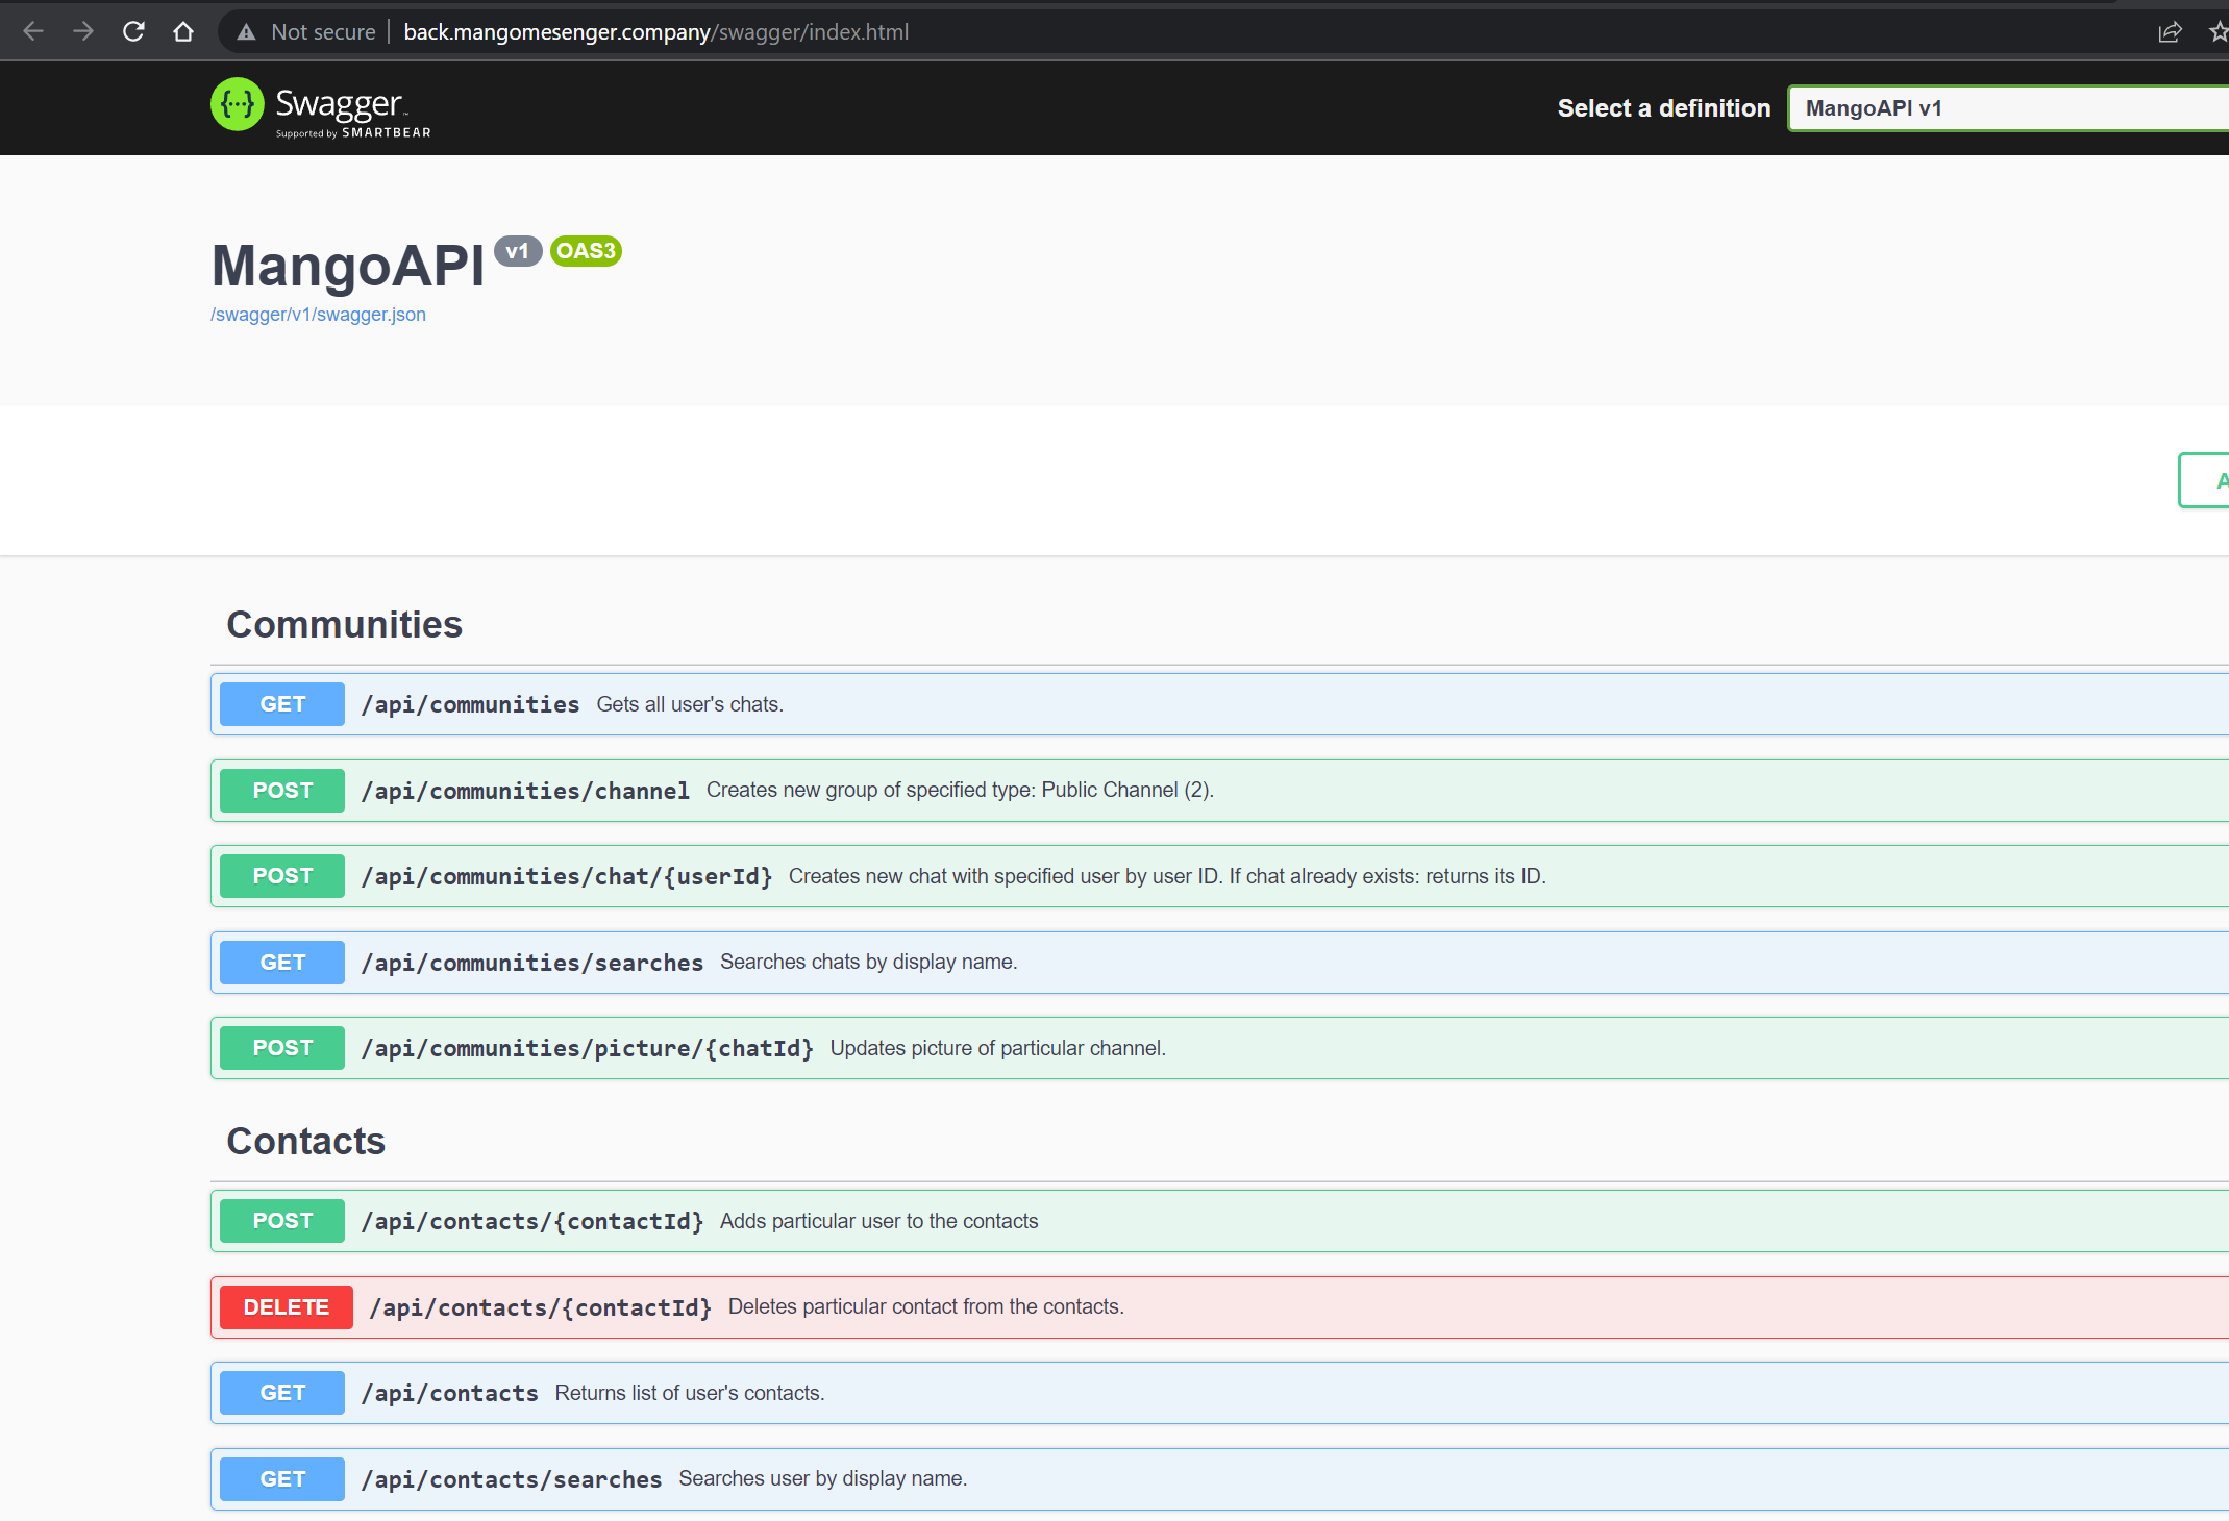
\includegraphics[width=1\textwidth]{img/07_swagger_under_domain_name}
    ~\caption{Application is available under the Domain name.}\label{fig:figure20}
\end{figure}

\subsection{Configure the HTTPS using LetsEncrypt Certbot}\label{subsec:configure-https-using-letsencrypt-certbot}
Configuring the \texttt{HTTPS} for our \texttt{nginx} server we are going to use the \texttt{CertBot} tool
from the \texttt{LetsEncrypt}.
We install it to the Ubuntu virtual machine using the following commands:
\begin{itemize}
    \item \texttt{sudo apt update -y}
    \item \texttt{sudo apt install -y python3 python3-pip python3-dev build-essential}
    \item \texttt{sudo pip3 install --upgrade pip}
    \item \texttt{sudo pip3 install certbot}
    \item \texttt{sudo pip3 install certbot-nginx}
\end{itemize}
A partial terminal output is as follows
\begin{figure}[H]
    \centering
    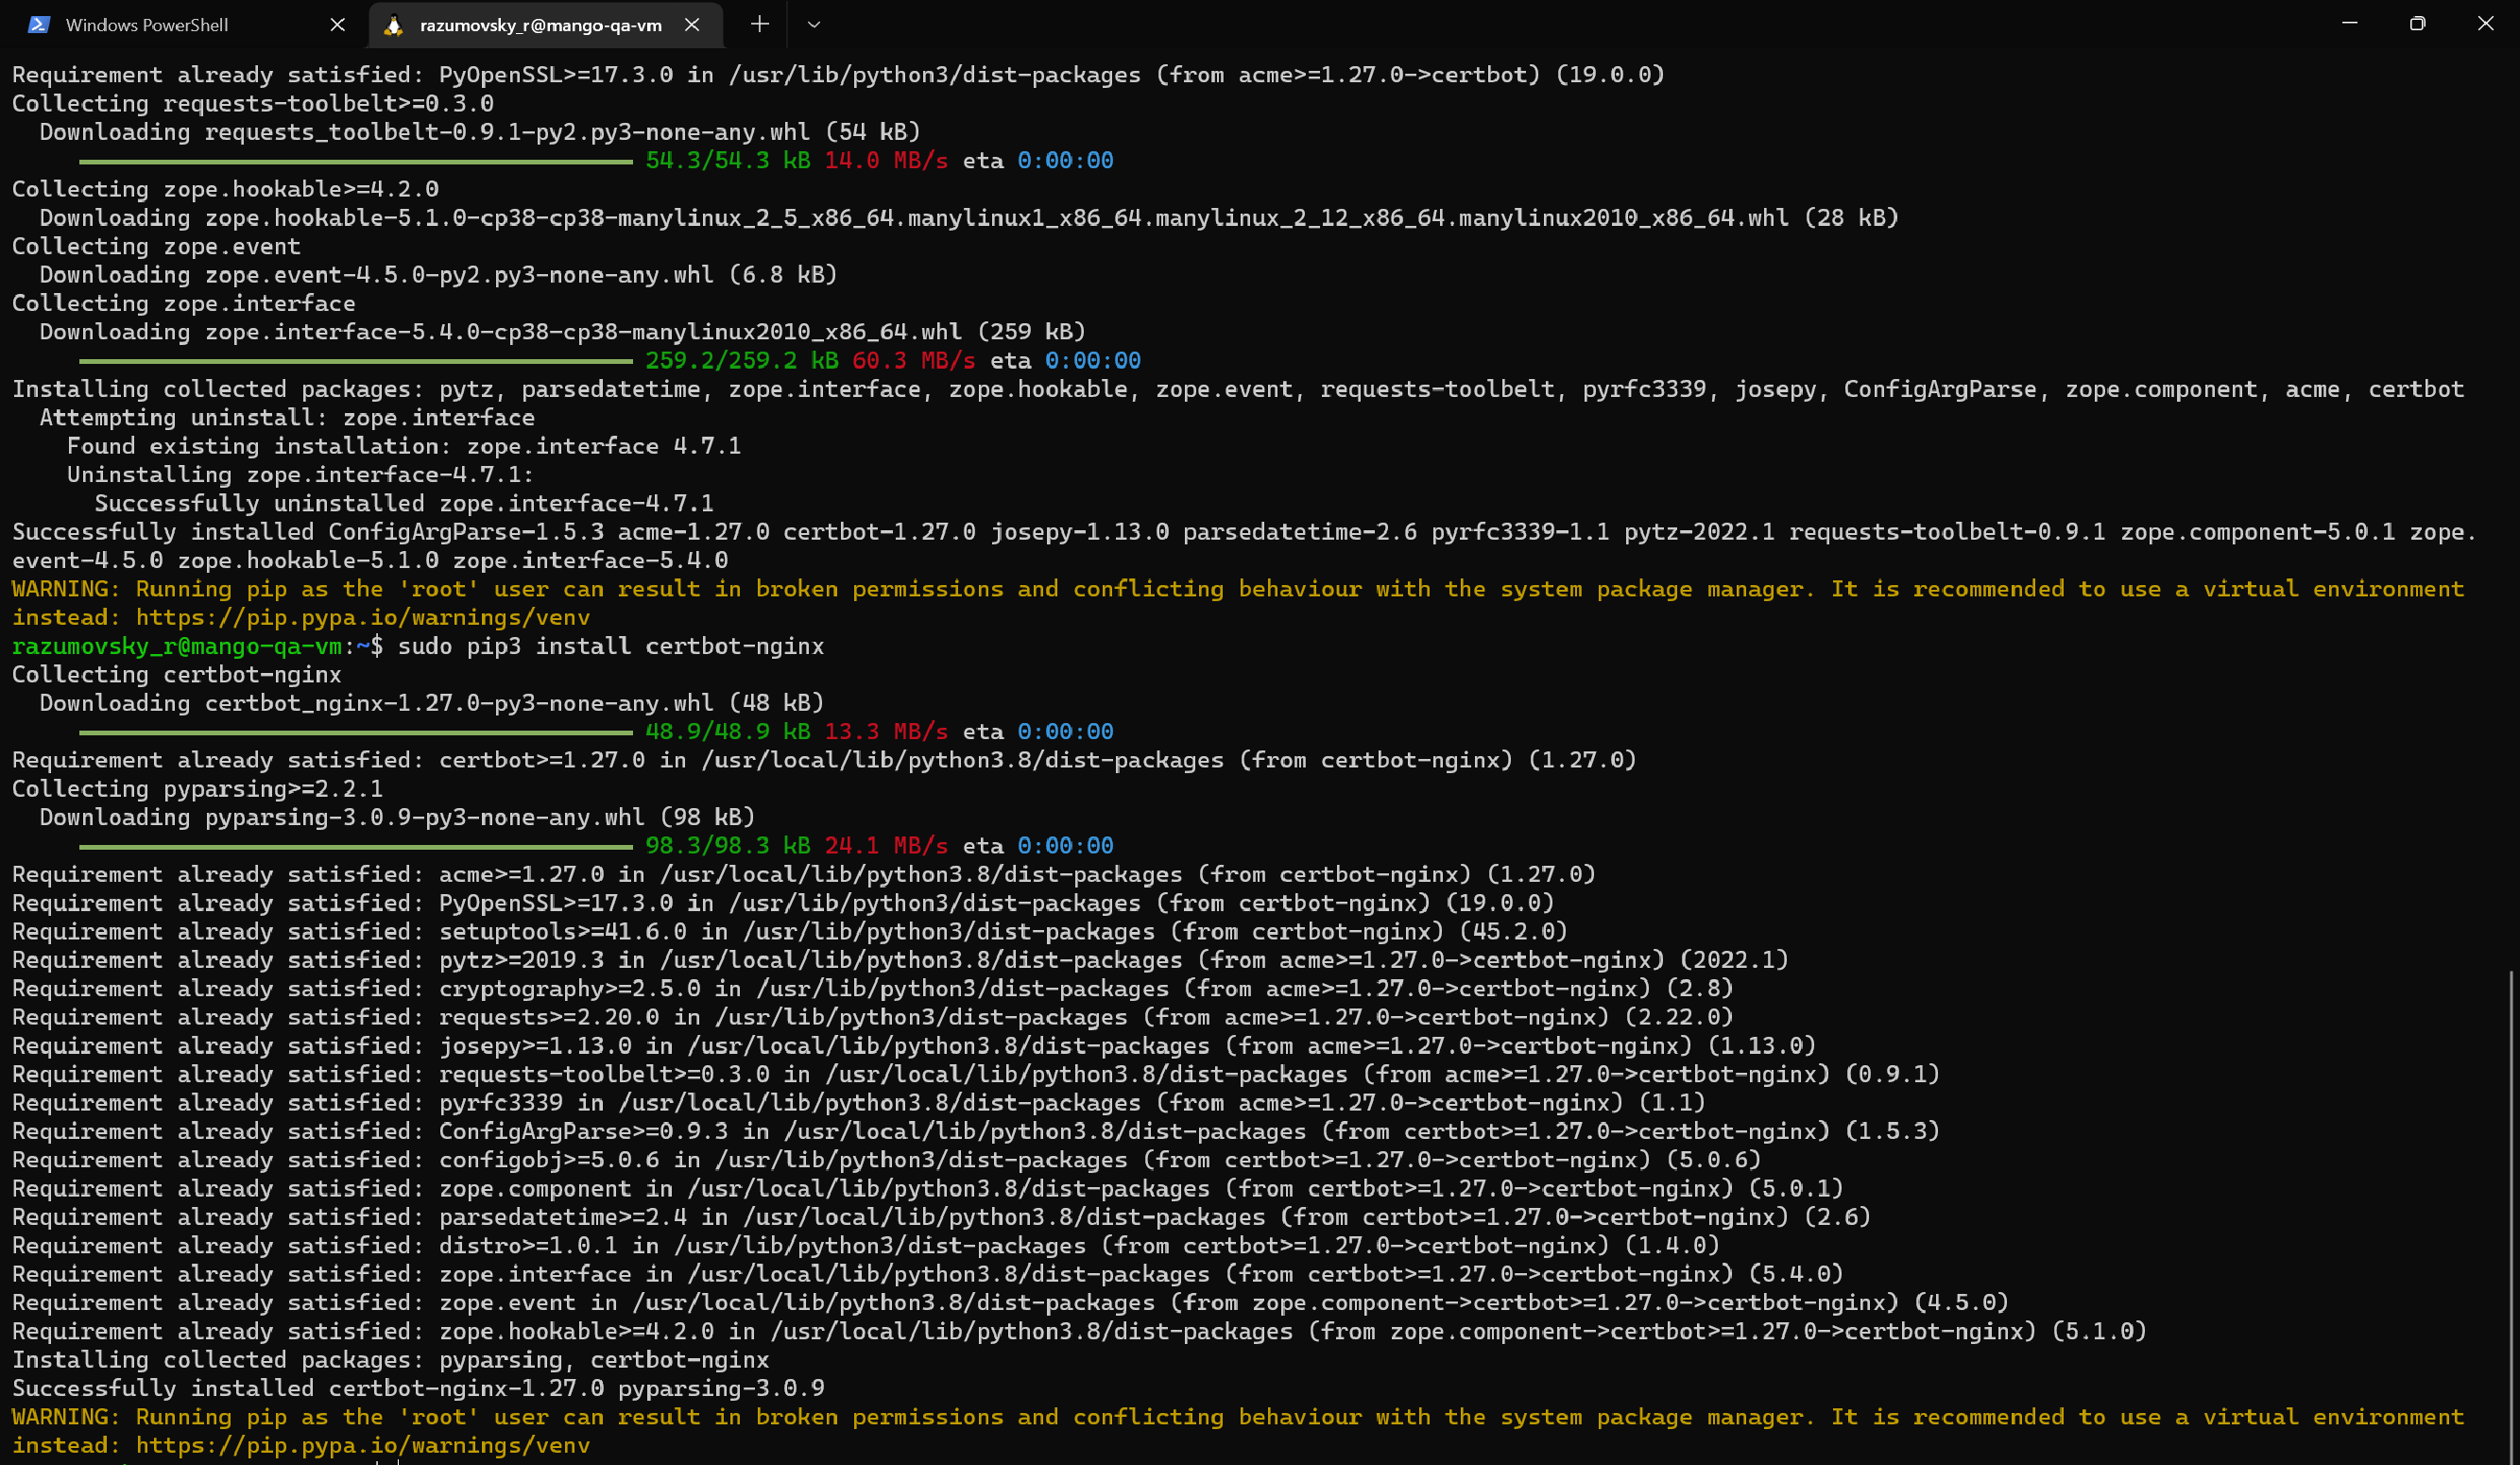
\includegraphics[width=1\textwidth]{img/07_install_certbot_console_output}
    ~\caption{Install \texttt{CertBot} tool terminal output.}\label{fig:figure21}
\end{figure}
Last part remaining is to certify out \texttt{nginx} web server so that it will accept \texttt{HTTPS} connections,
we do it using the commands:
\begin{itemize}
    \item \texttt{sudo certbot --nginx}
    \item \texttt{sudo systemctl restart nginx}
    \item \texttt{sudo nginx -t}
\end{itemize}
The terminal output is as follows
\begin{figure}[H]
    \centering
    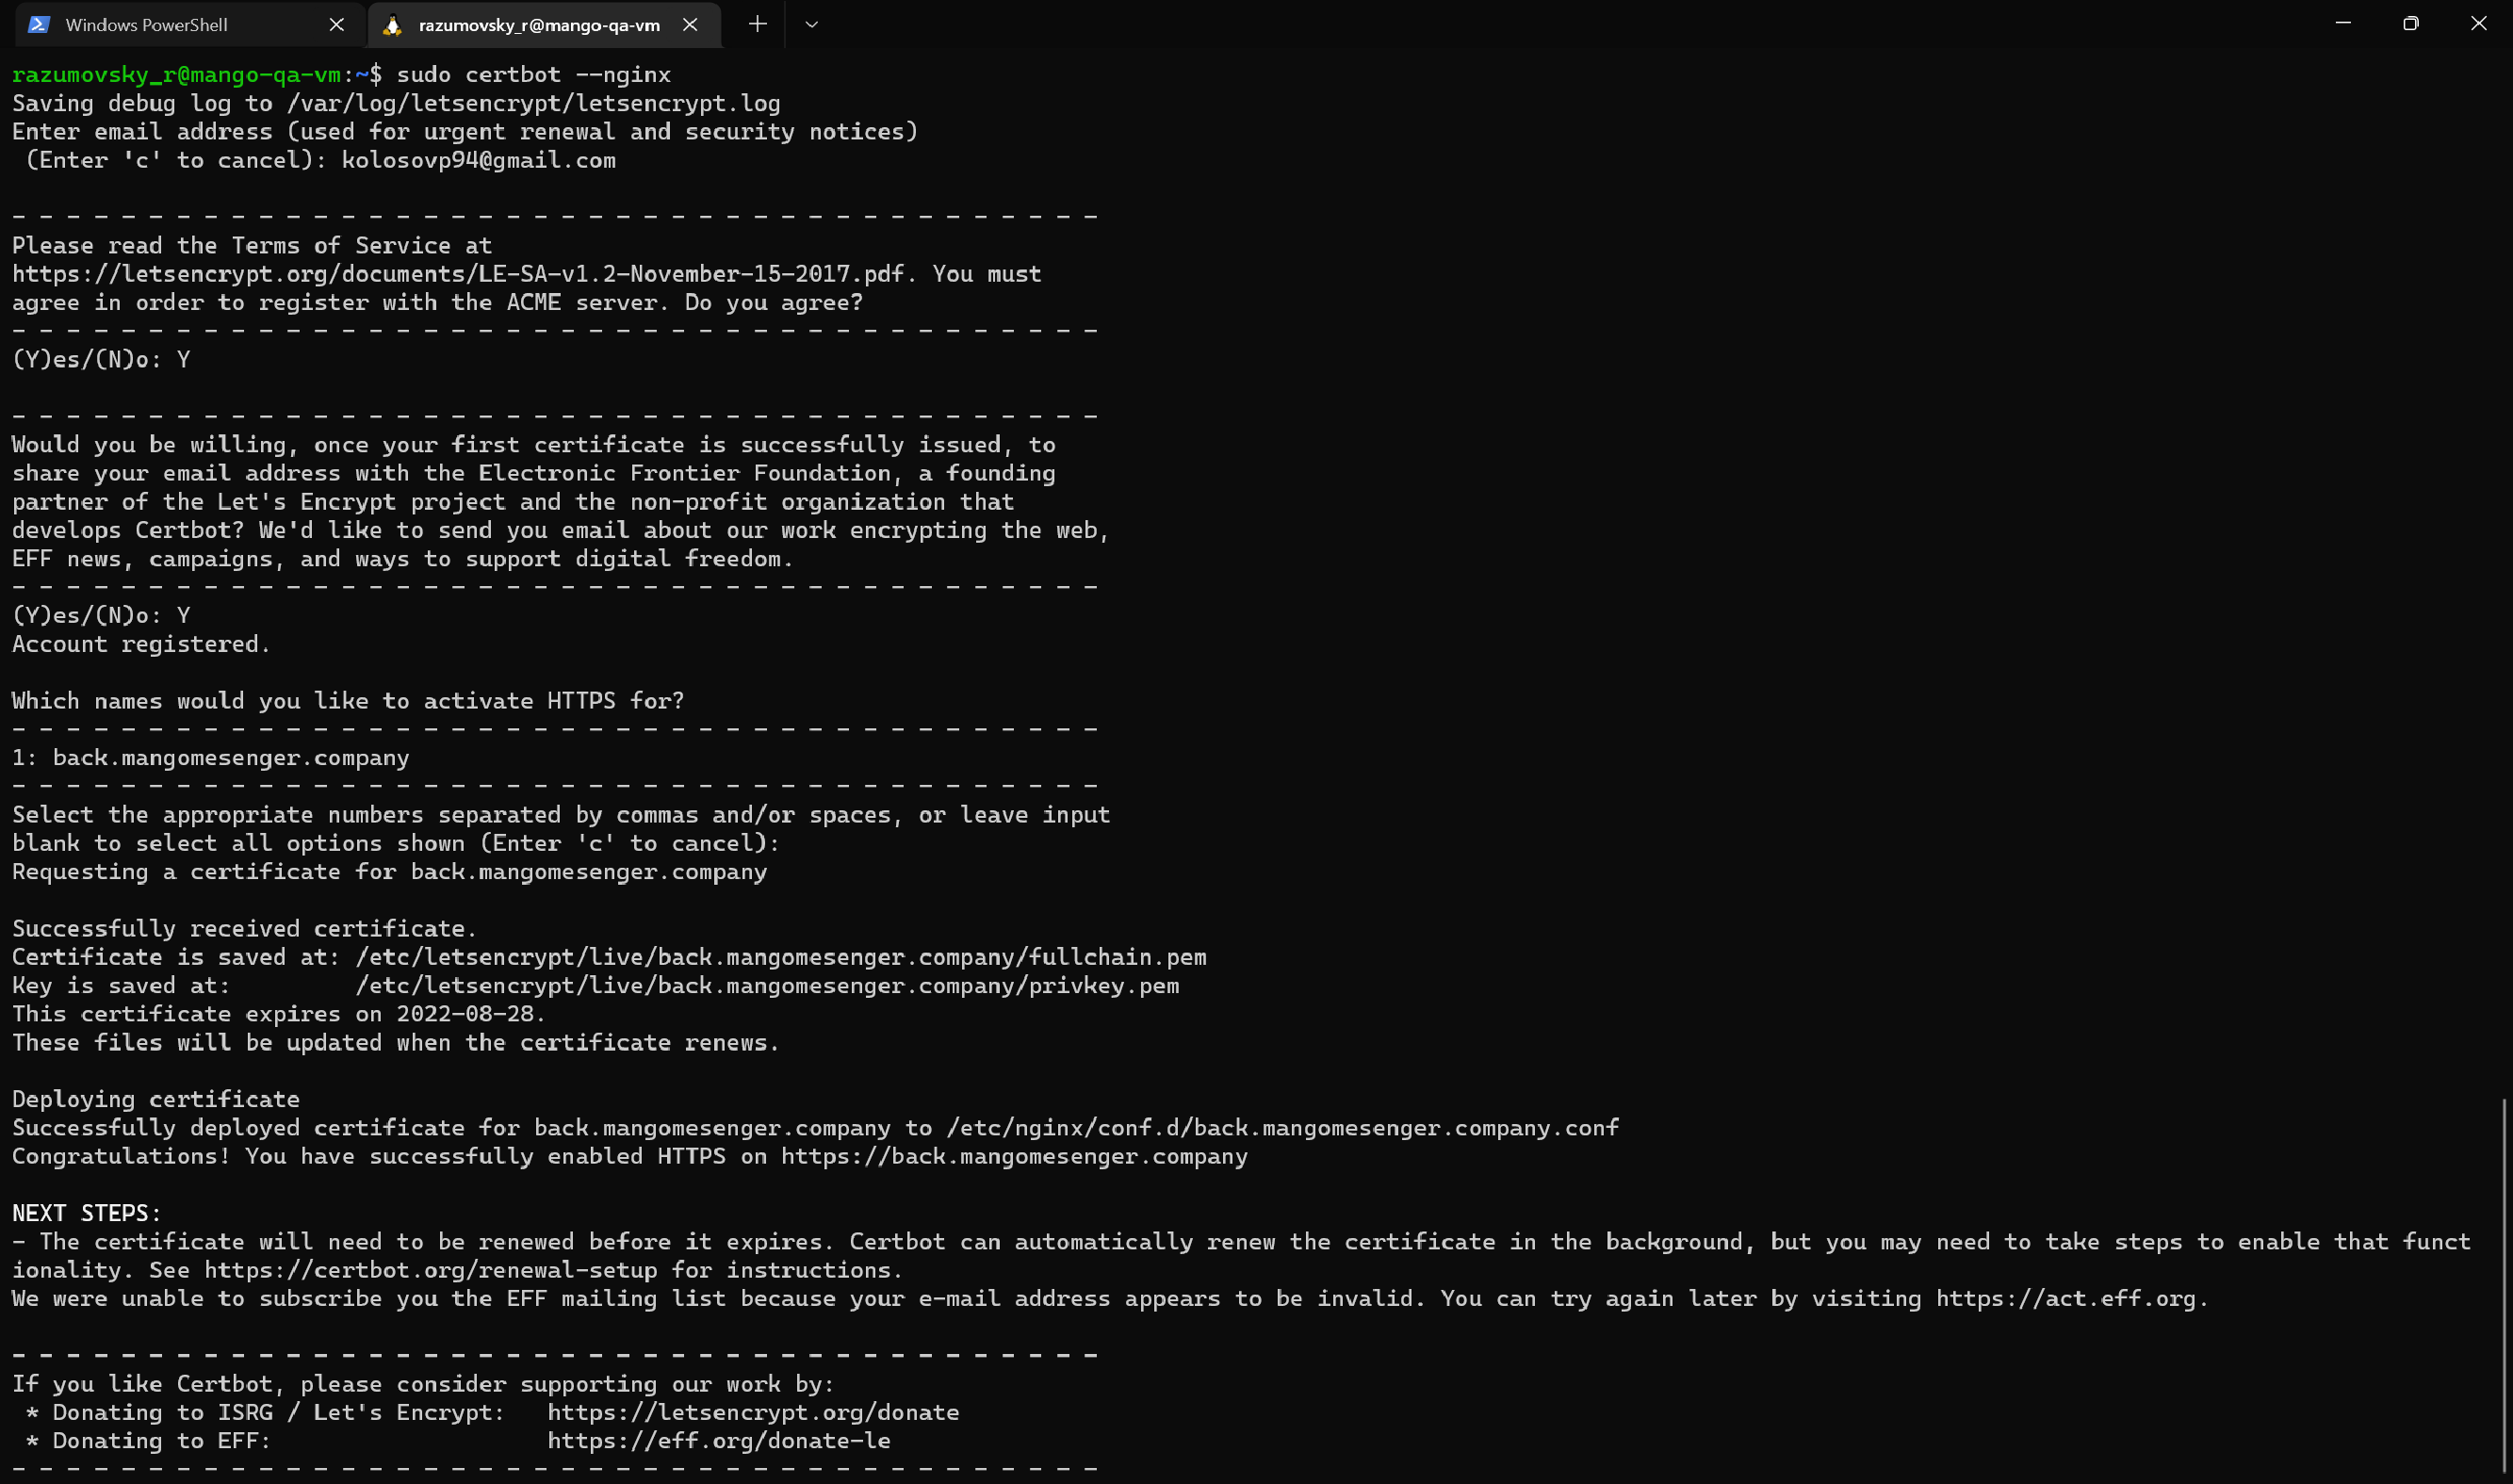
\includegraphics[width=1\textwidth]{img/07_certbot_nginx}
    ~\caption{\texttt{sudo certbot --nginx} terminal output.}\label{fig:figure22}
\end{figure}

Finally, our web application accepts the \texttt{HTTPS} connections now
\begin{center}
    \href{https://back.mangomesenger.company/swagger}{\texttt{https://back.mangomesenger.company/swagger}}
\end{center}
And certificate looks as follows
\begin{figure}[H]
    \centering
    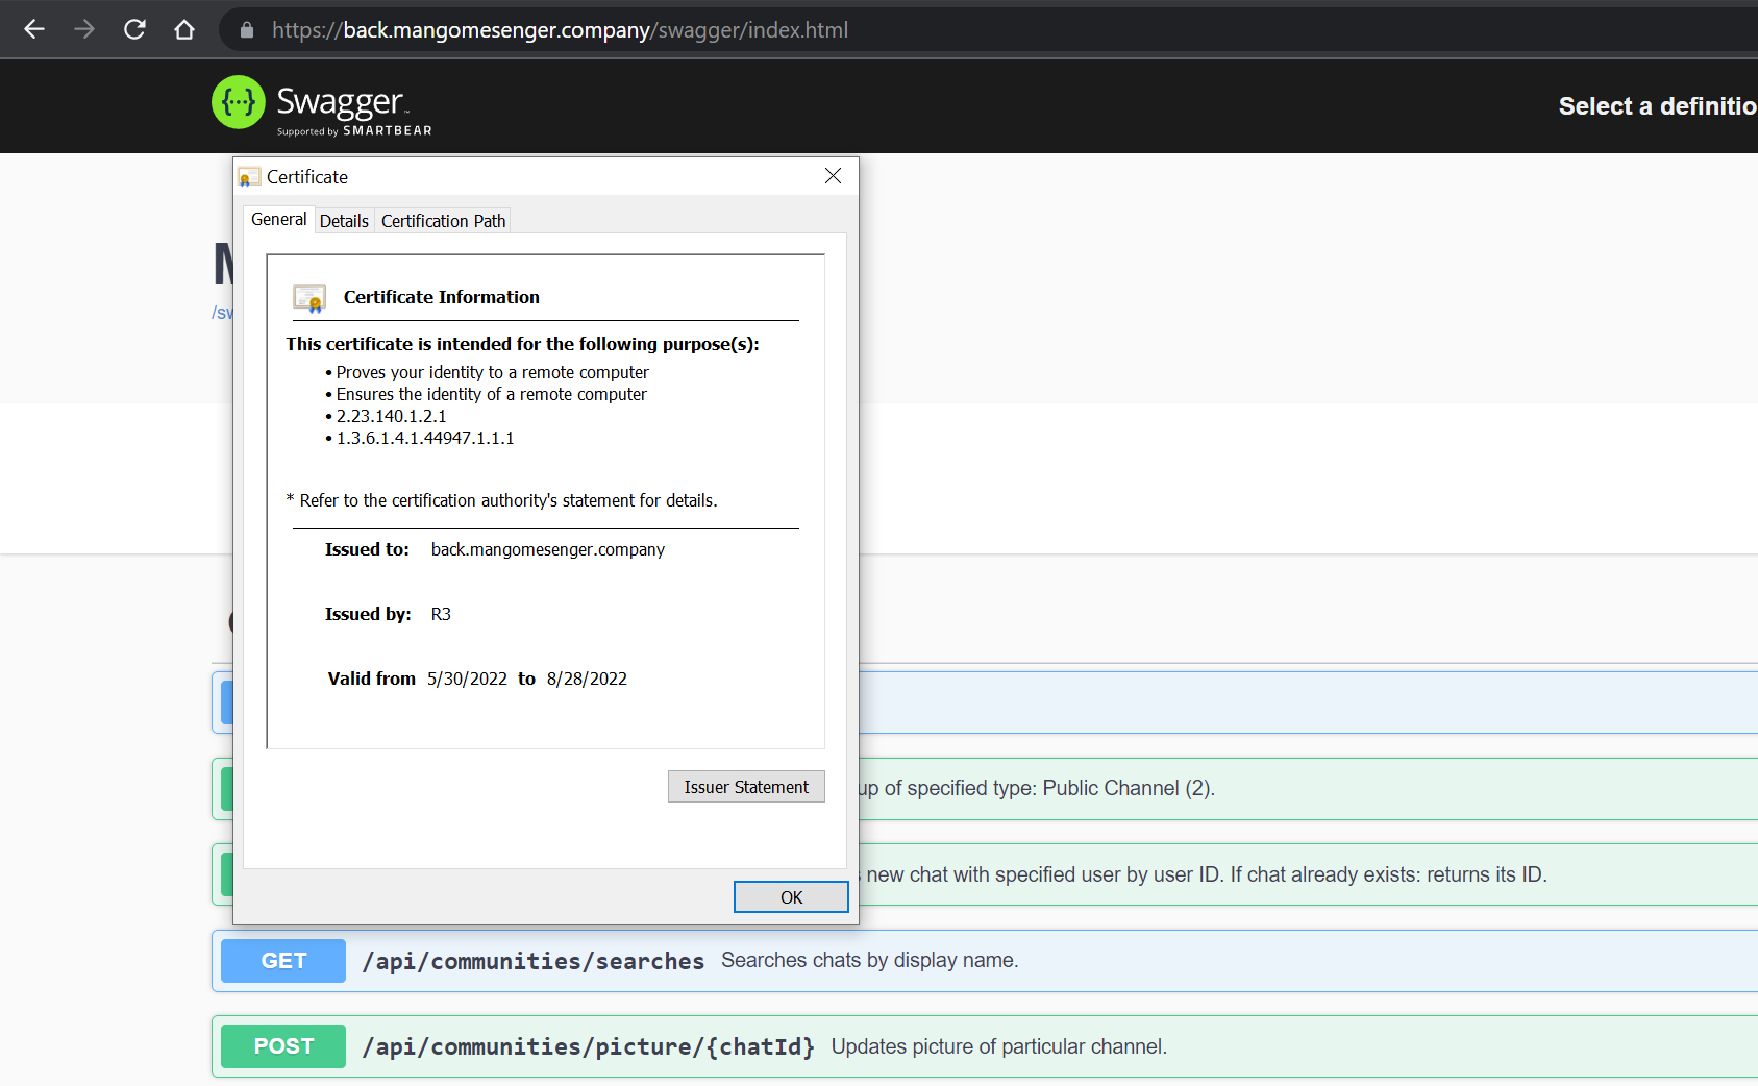
\includegraphics[width=1\textwidth]{img/07_https_browser_output}
    ~\caption{\texttt{sudo certbot --nginx} terminal output.}\label{fig:figure23}
\end{figure}
This completes the current section.



    \section{Conclusions}\label{sec:conclusions}
    We have reviewed ways to deploy ASP. NET Core Web API to the Ubuntu virtual machine using nginx server.
Also, we have bind vm under specified domain name and implemented HTTPS via lets encrypt certbot.

    \bibliographystyle{unsrt}
    \bibliography{AzureVMDeploy}
    \noindent \textbf{Version:} \texttt{Local-0.1.0}


\end{document}
